\documentclass{article}
\usepackage{ctex}
\usepackage{hyperref}
\usepackage{geometry}
\usepackage{amsmath}
\usepackage{caption}
\RequirePackage{longtable,multirow,array}
\RequirePackage{booktabs}
\usepackage{booktabs}
\usepackage{multicol}
\usepackage{longtable}
\usepackage{xurl}
\usepackage{booktabs}
\usepackage{algorithm}
\usepackage{algpseudocode}
\usepackage{enumitem}
\usepackage[style=ieee,sorting=nyt]{biblatex}
\assignrefcontextentries[]{*}
\addbibresource{References.bib}
\geometry{left=1in, right=1in, top=1in, bottom=1in}
\hypersetup{hidelinks}
\hypersetup{bookmarksnumbered=true,
	bookmarksopen=true,
	colorlinks=true,
	linkcolor=black,
	citecolor=blue,
	urlcolor=black}
\usepackage{tikz}
\usepackage{pgfplotstable}
\usepackage{pgfplots}
\pgfplotsset{compat=1.18}
\captionsetup{justification=centering}
\captionsetup[figure]{name={Fig.},labelsep=space,labelfont=bf}
\captionsetup[table]{name={Table},labelsep=space,labelfont=bf}
\CTEXoptions[today=old, contentsname=Contents]
\newcommand{\authyear}[1]{\citeauthor{#1} (\citeyear{#1})}
\setmainfont{Arial}

\newcommand{\toB}[1]{\color{blue}#1\color{black}}

\begin{document}
	\title{\vspace{-2.25cm} Multimodal Abnormity-Aware Model\\for Ocular Disease Diagnosis}
	\author{Siqi Pan}
	\date{}
	\maketitle
	
	\vspace{-0.2cm}
	\hrule
	\vspace{-0.1cm}
	\section*{Abstract}
	\hrule
	\vspace{0.4cm}
	We devise a novel model, the Multimodal Abnormity-Aware Model (MAAM), for assisting ocular disease diagnosis. The MAAM enables input of 2 kinds of ophthalmological images, namely optical coherence tomography (OCT) and color fundus images, and simulates the decision-making process by deducing the disease from abnormities. The model is composed of 2 submodels, the Abnormity Models and the Diagnosis Model, where the Abnormity Models identify 11 OCT abnormities and 8 fundus abnormities, and the Diagnosis Model identifies 12 diseases by integrating features from the former model. In MAAM, we introduce the fusion mechanics, the concept of codominant abnormities and diseases, and the Abnormity-to-Disease Criteria.  The model breaks the black box of complex neural network and expose more interpretable information for the reference of ophthalmologists. And it gets the overall accuracy of 89\% and thus the feasibility is verified.
	\vspace{0.4cm}
	\hrule
	\vspace{1cm}
	
	\begin{multicols}{2}
	\section{Background}
	Ocular diseases can be diagnosed through various methods, including using optical coherence tomography (OCT) and color fundus images. Ophthalmologists usually identify ocular abnormalities to deduce the disease. Traditionally, the diagnosis primarily depends on the professional experience and knowledge of the ophthalmologists, which may result in high misdiagnosis rate and under-utilization of medical data. With the widespread application of artificial intelligence (AI), deep learning (DL) has made great contributions in providing support to patients in remote areas by sharing expert knowledge \autocite{Ichhpujani_Thakur_2021}. By leveraging DL, researchers have developed auxiliary diagnosis programs to help ophthalmologists in the process. Many studies use convolutional neural networks (CNN) to analyze ocular images. Some commonly used CNNs are VGG, ResNet, and Inception \autocite{daich2023artificial}. And for segmenting images and finding abnormalities, U-net is widely used \autocite{Ronneberger_Fischer_Brox_2015}. With regards to training CNNs, most studies use transferred learning, which consists of three steps: learning, fine-tuning, and validation.
	
	Some studies directly predict the disease from OCT images.
	\authyear{li2019deep} used ResNet to analyze OCT images and distinguish between choroidal neovascularization (CNV), diabetic macular edema (DME), drusen, and healthy eyes. In addition, they performed occlusion testing to find out the regions that are the most important in diagnosis \autocite{li2019deep}. 
	\authyear{yoo2021feasibility} used generative adversarial network (GAN) and Inception-v3 together with a few-shot dataset to investigate the feasibility of improving OCT diagnosis of rare ocular diseases \autocite{yoo2021feasibility}. They handled the issues of training image shortage and data imbalance by creating ocular disease OCT images from healthy OCT images. \authyear{Kermany2018} conducts medical diagnosis and identifies treatable diseases by image-based deep learning. They also provided a widely used database including more than one hundred thousand OCT labeled images for 3 diseases \autocite{Kermany2018}.
	
	Some other studies can identify ocular abnormalities from annotated OCT images.
	\authyear{camino2018deep} used DL to identify the region of preserved photoreceptors on \textit{en face} OCT in choroideremia and retinitis pigmentosa (RP) \autocite{camino2018deep}. 
	\authyear{srinivasan2014fully} detected DME and dry age-related macular degeneration (dry AMD) from OCT images by flattening the image and using support vector machine (SVM) to extract the thickness information of the retinal layers \autocite{srinivasan2014fully}. 
	\authyear{leandro2023oct} implemented VGG to identify up to 8 kinds of key abnormalities and hence detect multiple diseases by using central fovea cross-section OCT \autocite{leandro2023oct}. \authyear{Fang_Wang2019} developed a novel lesion-aware CNN, called LACNN, to simulate the ophthalmologists' diagnosis that focuses on ocular abnormalities. The LACNN is a U-net-like CNN which incorporates VGG16 as the baseline, and the result is impressive \autocite{Fang_Wang2019}.
	
	Other studies use fundus images to predict ocular diseases.
	\authyear{masumoto2019accuracy} trained deep CNN with ultrawide-field fundus images to make the CNN capable of diagnosing RP \autocite{masumoto2019accuracy}. 
	\authyear{chen2021artificial} uses color fundus photographs and multiple types of CNN (Inception V3, Inception Resnet V2, and Xception) to develop a method of early detection of RP \autocite{chen2021artificial}. 
	\authyear{li2022development} uses CNN to detect up to 12 fundus diseases based on colour fundus photography \autocite{li2022development}. \authyear{Son2023} presented a novel architectural and algorithmic design to comprehensively identify 15 abnormalities and diagnose 8 major ocular diseases from macula-centered fundus images. They defined a notion of counterfactual attribution ratio (CAR) to interpret the system's diagnostic reason and disclose the relationship between abnormalities and diseases \autocite{Son2023}.
	
	In recent years, more and more DL systems began to use multi-modal information to predict ocular diseases. For automated detection system, retrieving features from both OCT images and fundus images can effectively keep the diagnosis away from bias and incompleteness. It is not always necessary to yield a better automated diagnosis result, but it does help ophthalmologist to make more accurate and holistic clinical decisions. For instance, \authyear{liu2023prediction} combined OCT and fundus images to evaluate visual impairment in RP in terms of best-corrected visual acuity(BCVA) \autocite{liu2023prediction}. \authyear{Xu2021} leveraged a bi-modal CNN to diagnose AMD and polypoidal choroidal vasculopathy (PCV), where the architecture uses fundus and OCT images as input for transferred learning CNN and concatenates the retrieved features to classify 3 diseases including dry AMD, wet AMD and PCV \autocite{Xu2021}. And \author{Andrearczyk2018} ingeniously combined medical images and biomedical textual information to discriminate different diseases, which is a novel method for the usage of multi-modal application \autocite{Andrearczyk2018}.
	
	The key technical problem of multi-modal diagnosis is how to fuse the results from multifarious sources. There are three types of fusion, namely early, late, and hybrid fusion. Deciding on the optimal type of fusion is part of the exploratory process in the application of DL methods \autocite{Ichhpujani_Thakur_2021}.
	
	\section{Overview}
	\label{sec:overview}
	
	We develop the Multimodal Abnormity-Aware Model (MAAM) to aid ophthalmologists in diagnosing ocular diseases. It considers both OCT and color fundus image inputs. In addition, it simulates the decision-making process of ophthalmologists when they examine patients, namely, first identifying the abnormities, and then deducing the disease. The model is designed in a way that partly opens up the ``black box'' of DL and presents more interpretable information to ophthalmologists for the reference. 
	
	The structure of the MAAM is shown in Fig.~\ref{fig:3_parts}. It consists of 2 submodels: the Abnormity Model and the Diagnosis Model. We input multiple OCT and fundus images to the Abnormity Models, and output the classification of abnormities as an input to the Diagnosis Model, which yields disease probabilities as the final result.
	
	\vspace{0.5cm}
	
	The Abnormity Models are de facto classifiers for abnormities, which are symptoms that can be directly observed in the images. The MAAM identifies 11 OCT abnormities and 8 Fundus abnormities, as shown in Fig.~\ref{fig:OCT_abnormities} and Fig.~\ref{fig:fundus_abnormities}. The abbreviations and detail information of abnormities and diseases are tabulated in ``Appendix''.
	
	\end{multicols}

	\begin{figure}[htbp]
	\centering
	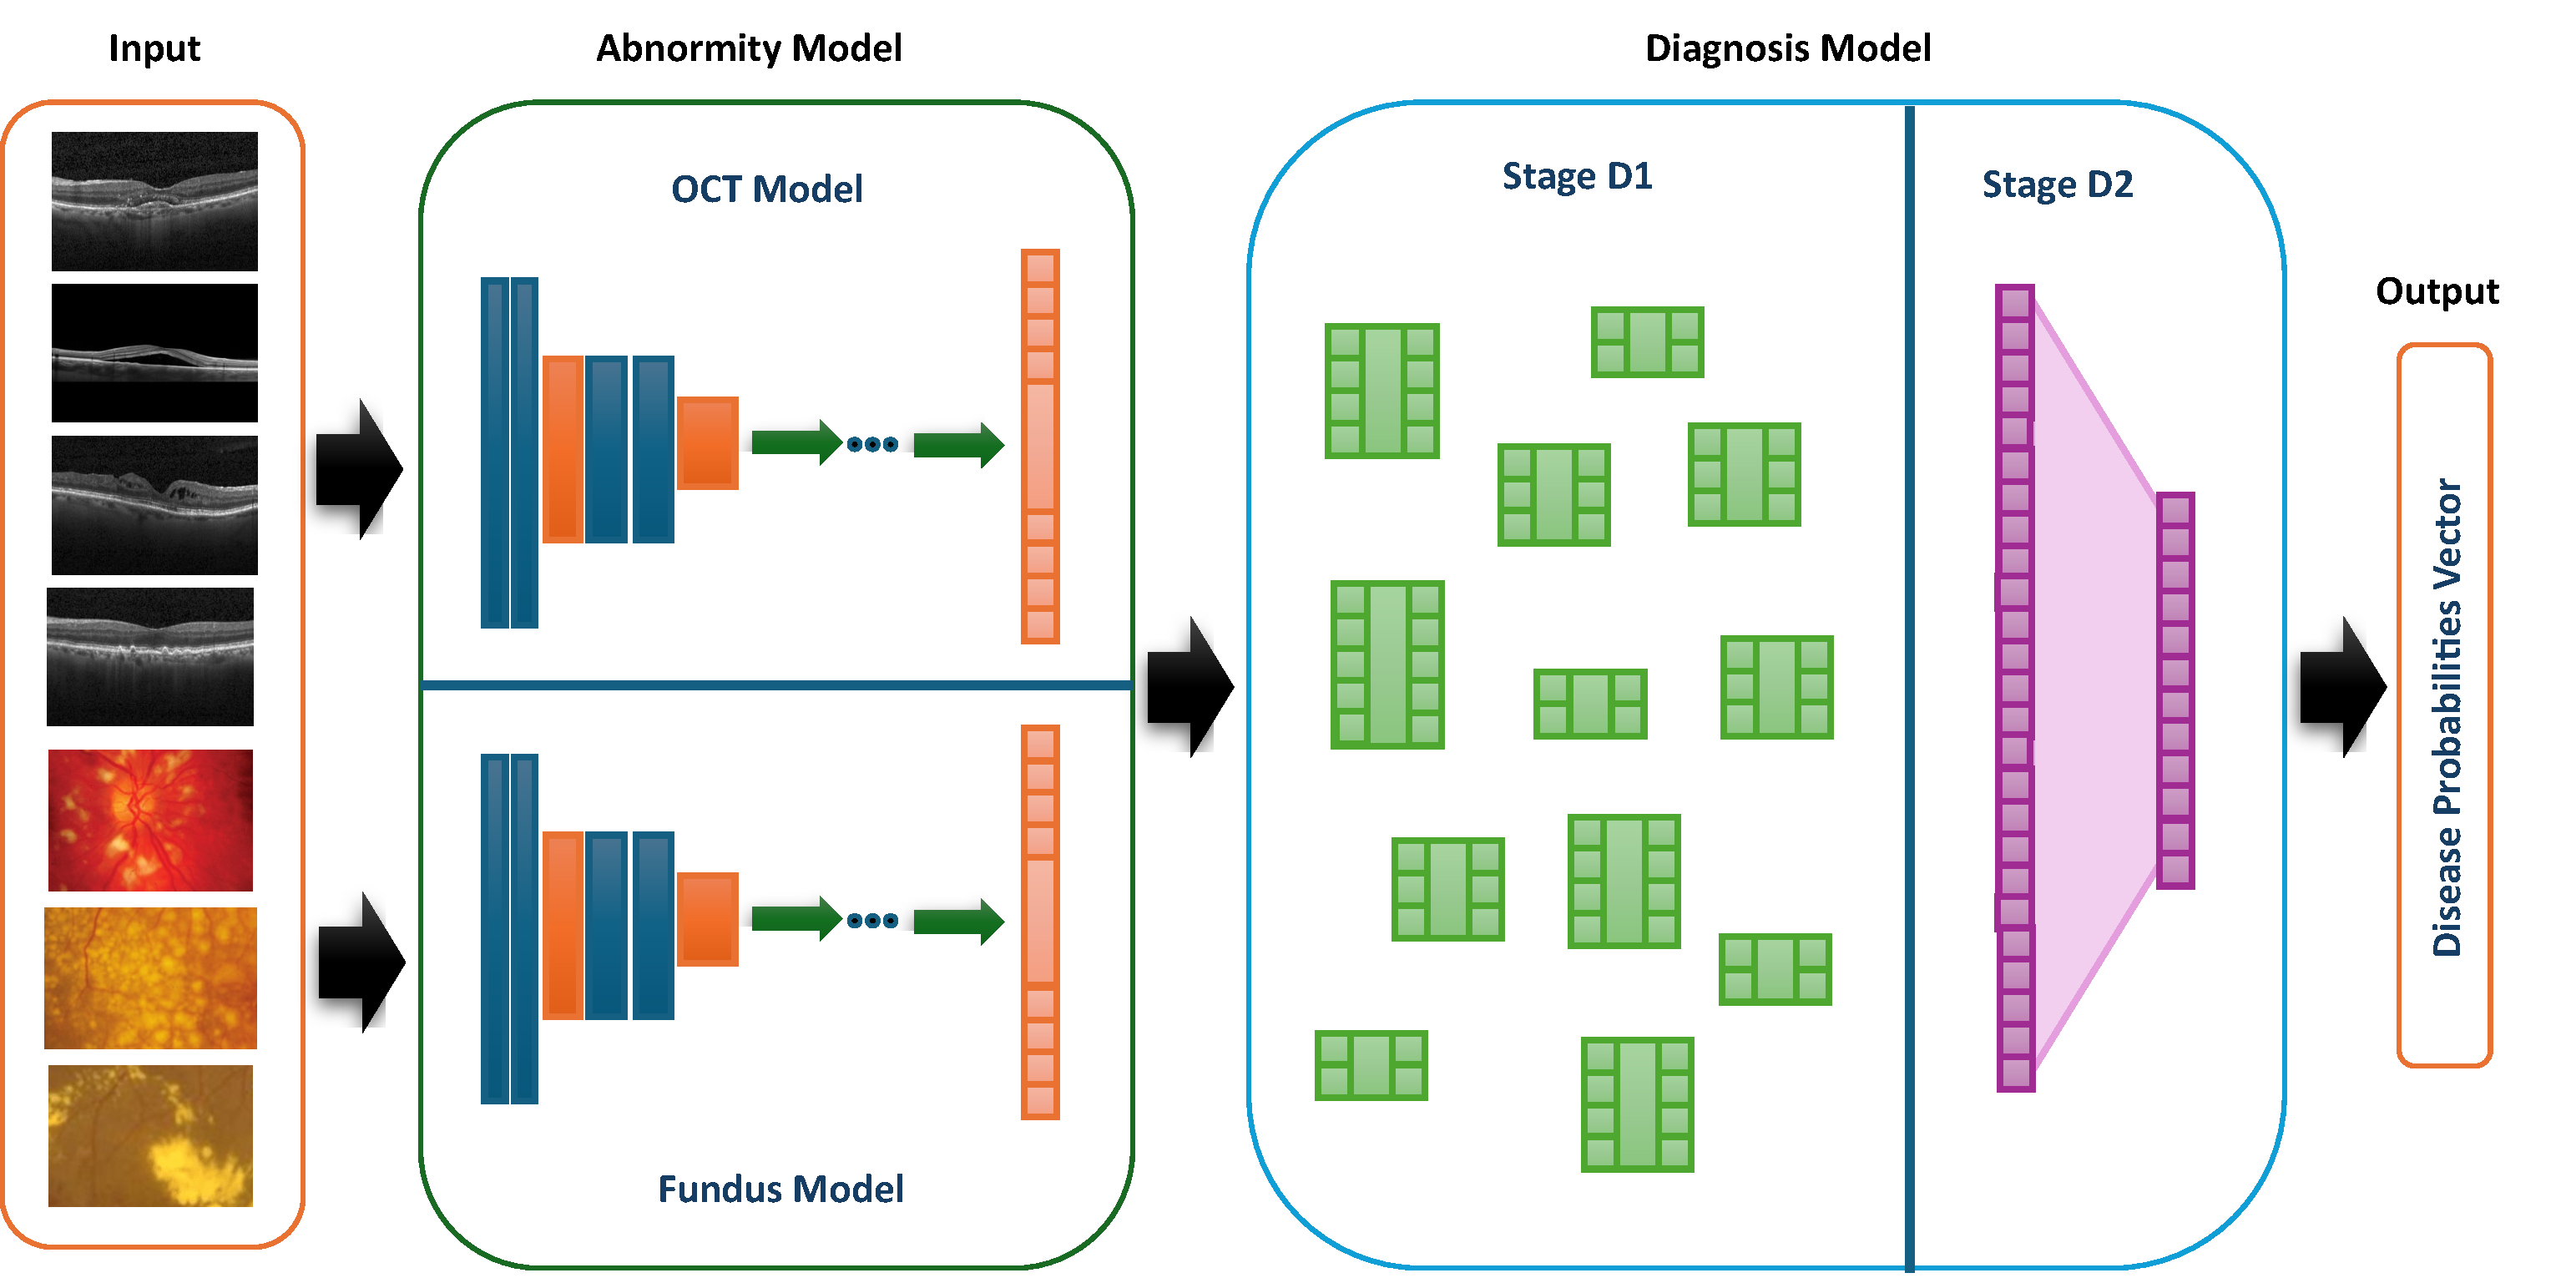
\includegraphics[width=\linewidth]{Figs/model_overview.pdf}
	\caption{Model Overview}
	\vspace{0.3cm}
	\label{fig:3_parts}
	\end{figure}


	
	\begin{figure}[htbp]
		\centering
		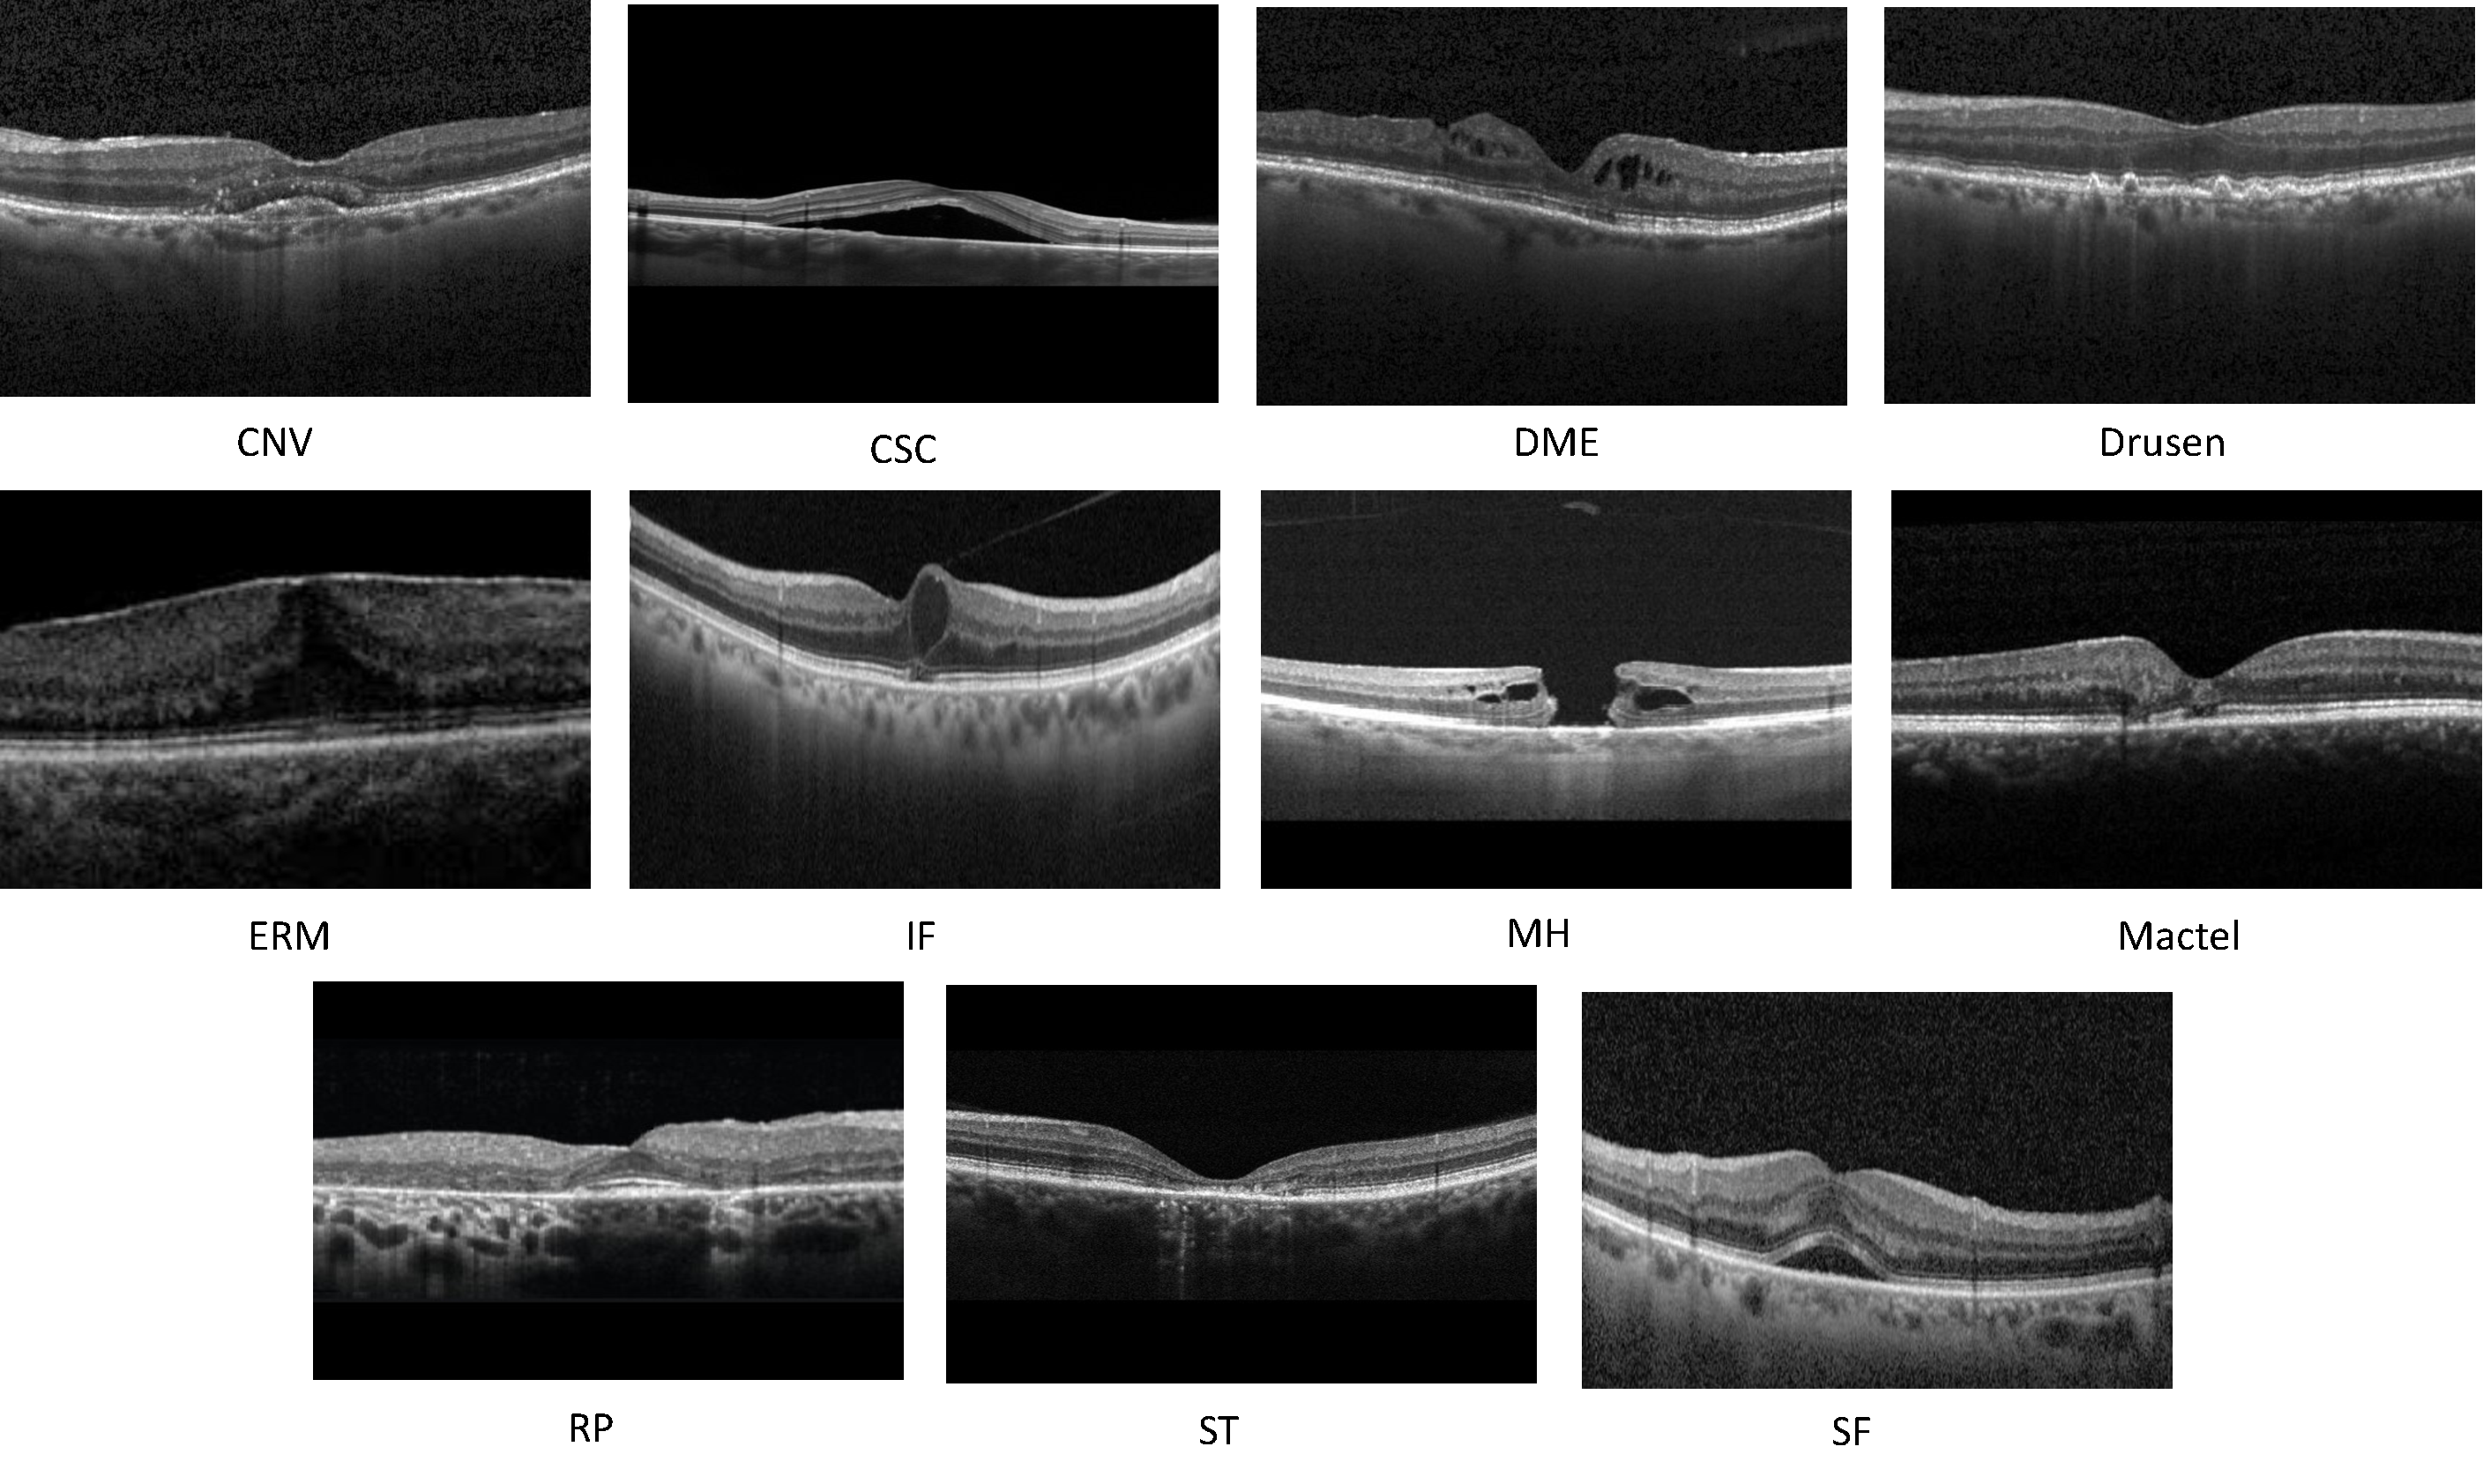
\includegraphics[width=\linewidth]{Figs/OCT_Abnormities.pdf}
		\caption{OCT Abnormities \autocite{Duker_Waheed_Goldman_2022}}
		\vspace{0.3cm}
		\label{fig:OCT_abnormities}
	\end{figure}
	
	\begin{figure}[htbp]
		\centering
		\includegraphics[width=\linewidth]{Figs/fundus_Abnormities.pdf}
		\caption{Fundus Abnormities \autocite{Wolf_Kirchhof_Reim_2006}}
		\vspace{0.3cm}
		\label{fig:fundus_abnormities}
	\end{figure}
	
	\begin{multicols}{2}
		
	The Abnormity Models also contain 2 submodels: the OCT Model and the Fundus Model, which classify OCT and fundus abnormities, respectively. Both of the submodels leverage CNNs with modified final fully-connected (FC) layers. We compare the performances of 4 commonly used CNNs, ResNet152, ResNet50, ResNet18 \autocite{He_Zhang_Ren_Sun_2016} and VGG16 \autocite{Simonyan_Zisserman_2015}, and choose the best one for each submodel. The final FC layer in each CNN is modified so that the size of its output vector is equal to the number of OCT or fundus abnormities. In order to normalize the output vector, we perform the softmax operation. Each submodel outputs a probability vector for all the abnormities.
	
	\vspace{0.5cm}
	
	The Diagnosis Model consists of two stages: Stage D1 and Stage D2. 
	
	\vspace{0.2cm}
	
	In Stage D1, we determine the severity level for each disease from the probability vectors from the Abnormity Models. We use Abnormity-to-Disease Deduction Criteria (shown in Fig.~\ref{fig:criteria}) as ground truth. There are multiple submodels in Stage D1 and each one corresponds to one disease. Based on the deduction criteria, we determine the number of abnormities for one disease and use the number to define the severity levels. For example, there are totally 5 abnormities that are present in the disease ``rDR'': OCT abnormity ``DME'' and Fundus abnormities ``HM'', ``VA'', ``MA'', and ``CWP''. Therefore, taking into account the healthy status, we end up with 6 severity levels for disease ``rDR''.

	We use the fused vector as an input for each submodels in Stage D1, and have the vector go through a FC layer with softmax operation to yield severity level probability vectors.
	
	\end{multicols}
	
	\begin{figure}[htbp]
		\centering
		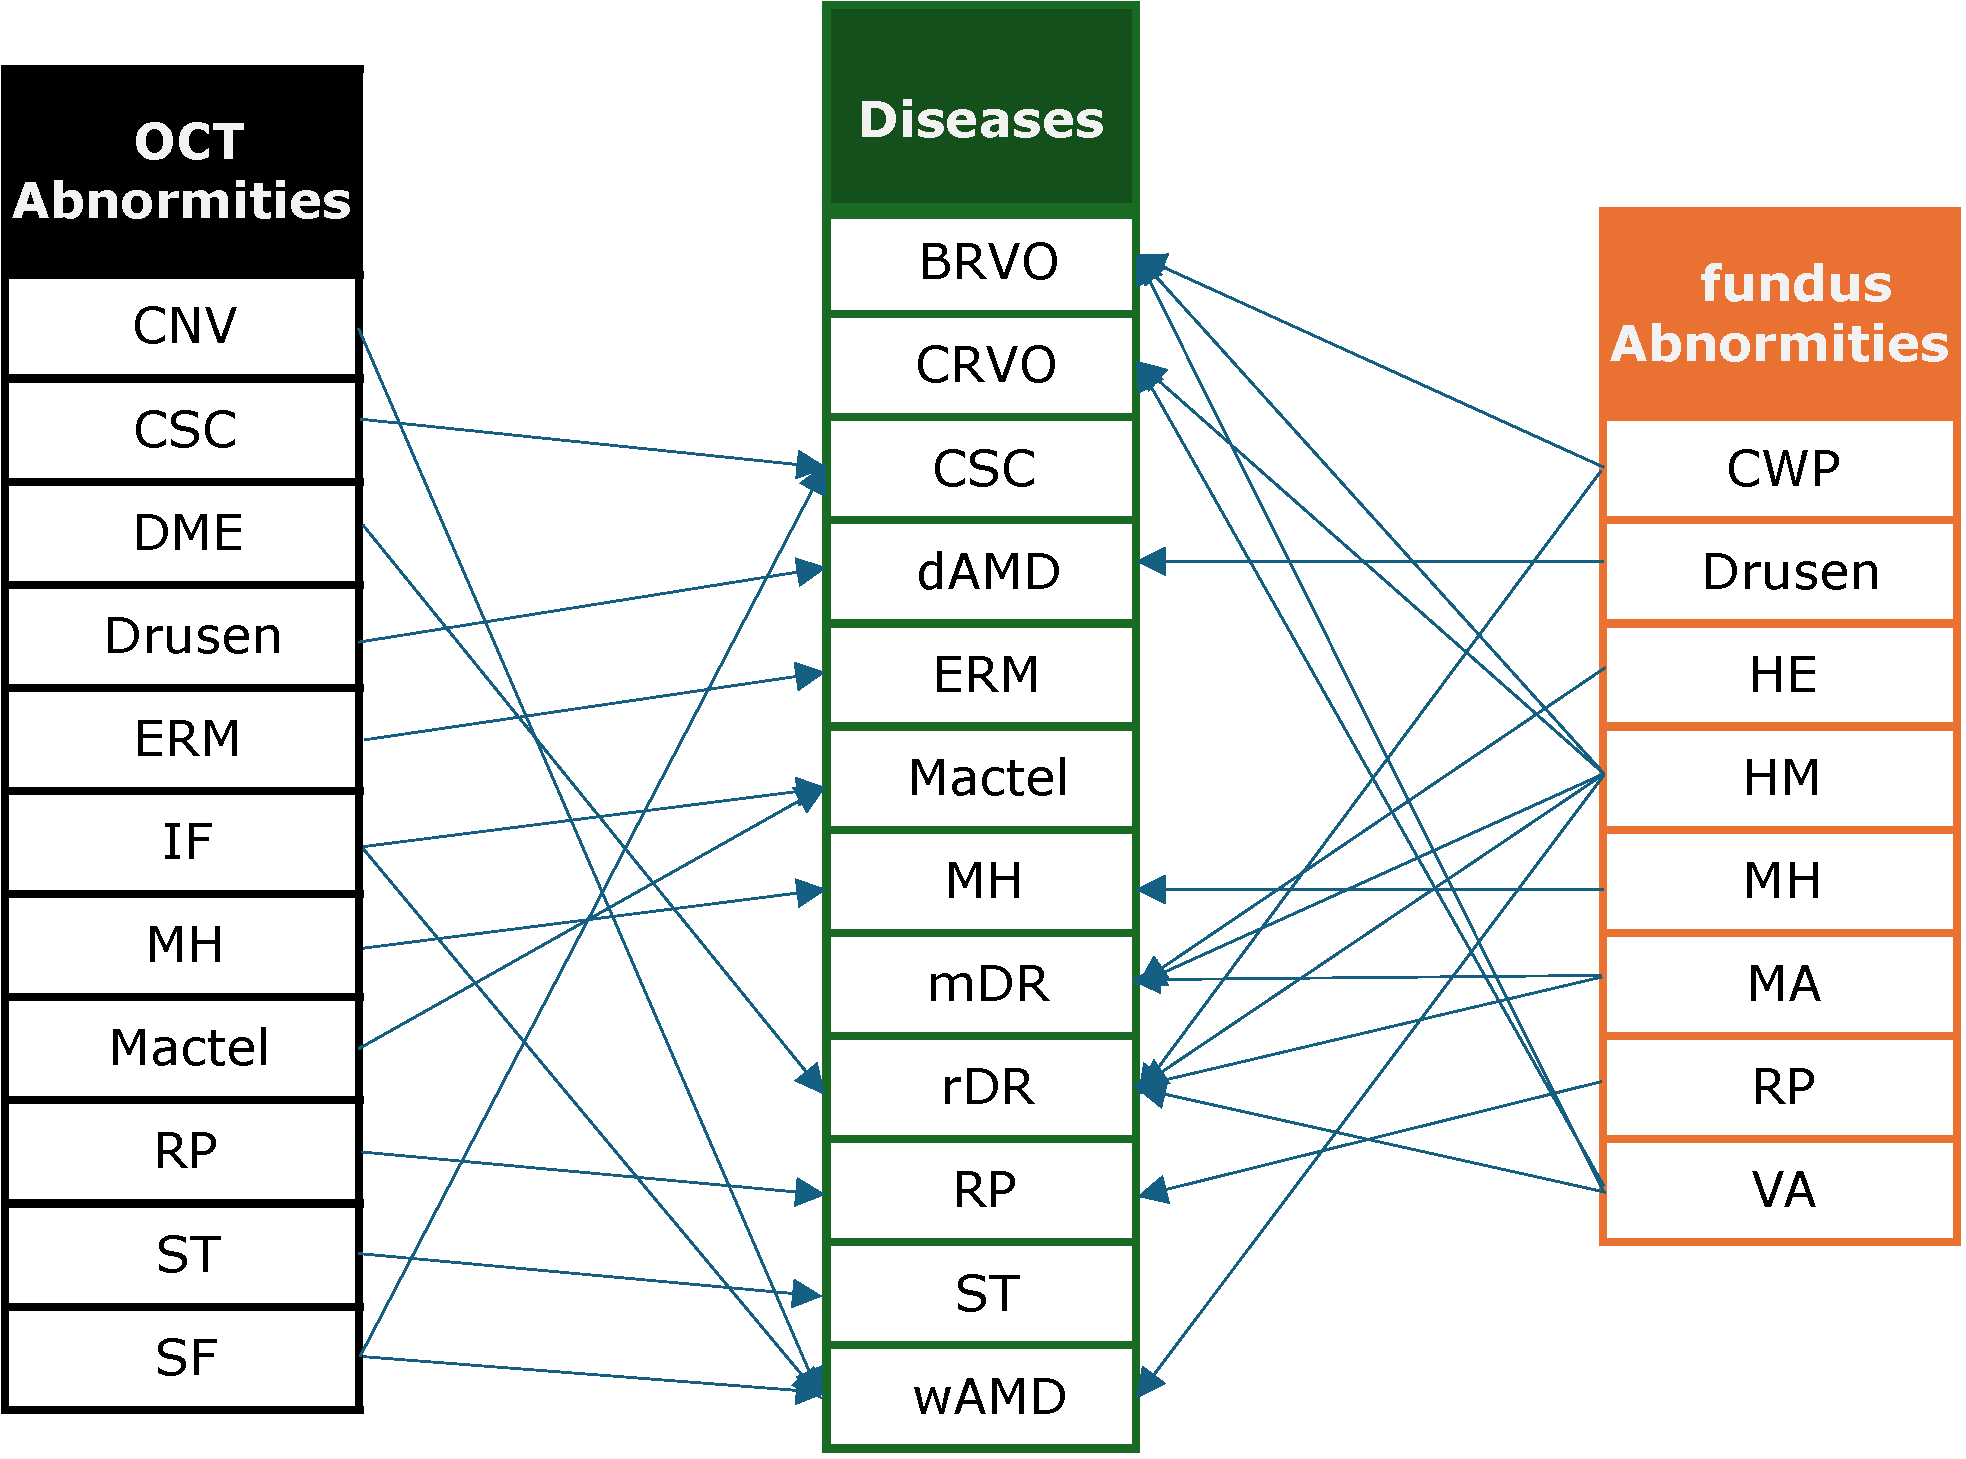
\includegraphics[width=0.8\linewidth]{Figs/criteria.pdf}
		\caption{Abnormity-to-disease Deduction Criteria}
		\vspace{0.3cm}
		\label{fig:criteria}
	\end{figure}

	\vspace{0.2cm}
	
	In Stage D2, we determine the final disease probability vector. Similarly, we use a fused vector from the outputs of submodels in Stage D1, and have the vector go through a FC layer with softmax operation. The result presents potential diseases that can be referenced by ophthalmologists.

	\vspace{0.5cm}
	
	In the MAAM, we leverage the fusion operation to incorporate all the results from different submodels. As shown in Fig.~\ref{fig:fusion}, there are totally 3 fusion operations in MAAM.
	
	\begin{figure}[htbp]
		\centering
		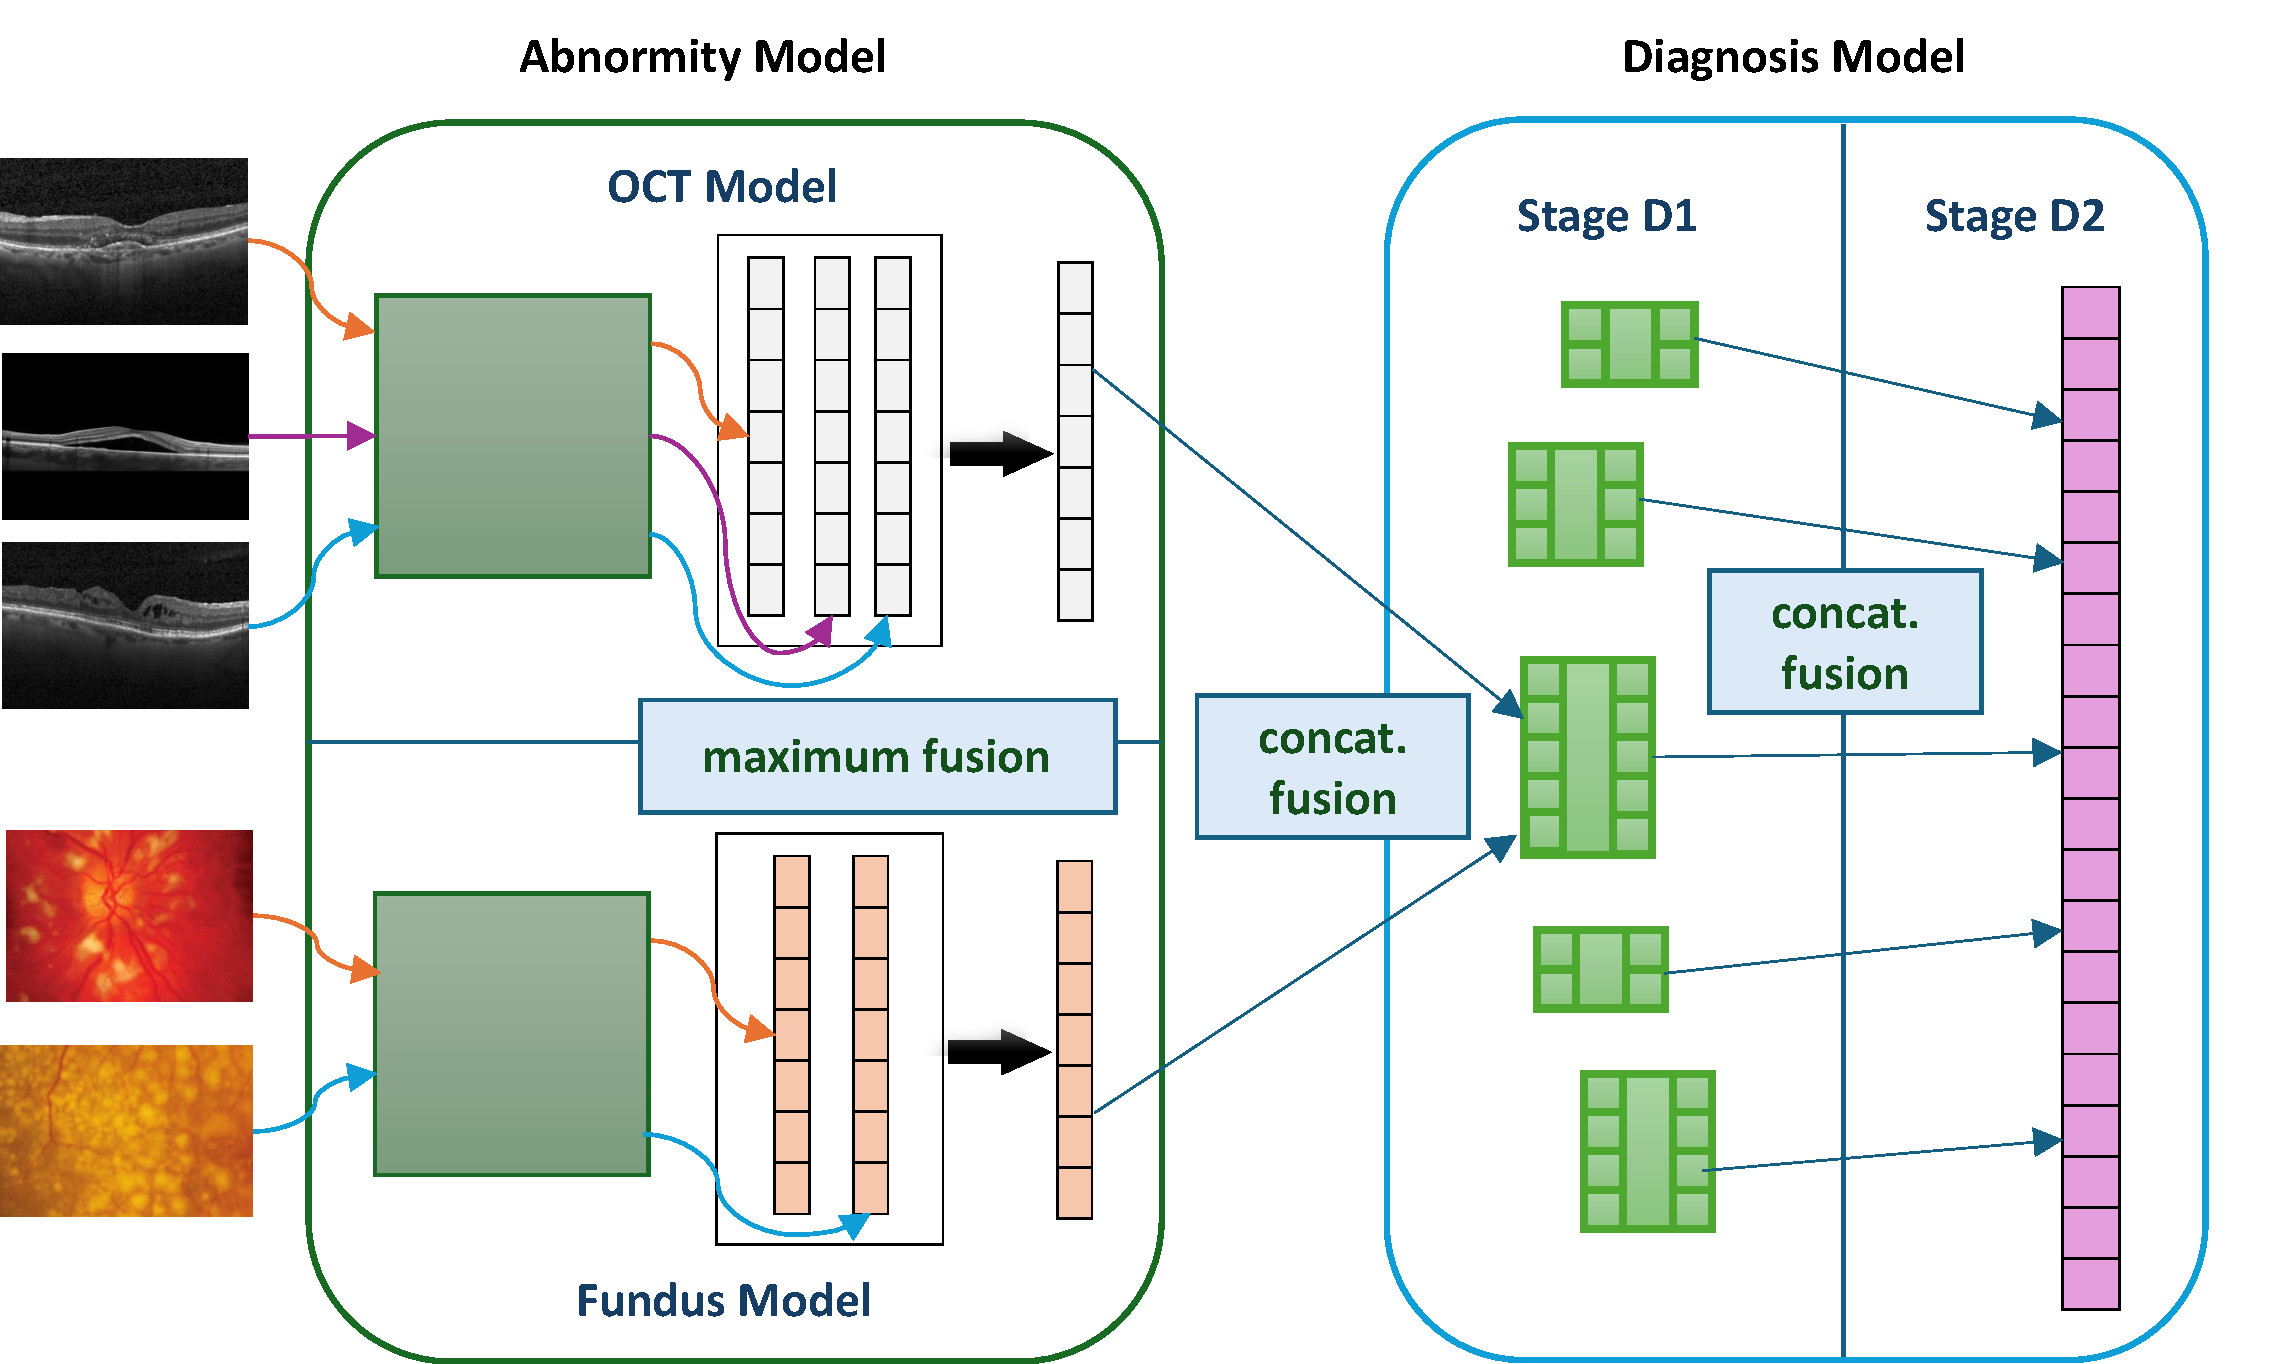
\includegraphics[width=\linewidth]{Figs/fusion.pdf}
		\caption{Fusion}
		\vspace{0.3cm}
		\label{fig:fusion}
	\end{figure}

	The first fusion occurs at the output of OCT Model or Fundus Model. In real scenarios, multiple OCT and Fundus images can be used for ocular disease diagnosis. Each image goes through either the OCT Model or the Fundus Model to yield a probability vector. To use the probability results from all the images, a maximization fusion is implemented for all the vectors so that the fusion yields one OCT abnormity probability vector and one Fundus abnormity probability vector with maximum values.
	
	The second fusion occurs at the interface between Abnormity Model and Stage D1. A concatenation fusion is implemented for OCT abnormity probability vector and Fundus abnormity probability vector. The fused vector works as an input to all the submodels in Stage D1.
	
	The third fusion occurs at the interface between Stage D1 and Stage D2. We concatenation all the severity level vectors to feed the model in Stage D2. The fused vector goes through the FC layer and undergoes a softmax operation to yield the final result.
	

	\section{Abnormity Models}
	
	\subsection{Data Preparation}
	
	The images and labels used for training are mainly downloaded from public databases, but some abnormities are not included in these databases. For those abnormities, we use the search engine as an additional data source to get images. The numbers of images acquired from each data source are shown in Table~\ref{tb:OCT_source} and Table~\ref{tb:Fundus_source}. As to the links of the images from the search engine, refer to ``Appendix''. 
	
	\begin{minipage}[t]{0.4\linewidth}
		{
			\fontsize{9}{12}\selectfont
			{
				\begin{longtable}{cccccc}
					\caption{OCT abnormities}
					\label{tb:OCT_source}\\
					\toprule
					\multirow{2}{*}{Abnormity}&\multicolumn{4}{c}{Source}&\multirow{2}{*}{Total}\\
					&1&2&3&4&\\
					\midrule
					CNV    &2984&-  &- &- &2984\\
					CSC    &-   &102&32&- &134 \\
					DME    &2500&-  &- &- &2500\\
					Drusen &2500&-  &- &- &2500\\
					ERM    &-   &-  &- &16&16  \\
					IF     &1097&-  &- &- &1097\\
					MH     &-   &99 &31&- &130 \\
					Mactel &-   &-  &29&- &29  \\
					Healthy&5000&-  &- &- &5000\\
					RP     &-   &102&31&- &133 \\
					ST     &-   &-  &23&- &23  \\
					SF     &1083&-  &- &- &1083\\
					\bottomrule
				\end{longtable}
				
				\vspace{0.5cm}
				\begin{enumerate}
					\item Normal Disease Database \autocite{Kermany_database}
					\vspace{-0.2cm}
					
					\item OCTID \autocite{Gholami_Roy_Parthasarathy_Lakshminarayanan_2020}
					\vspace{-0.2cm}
					
					\item Few-shot \autocite{Yoo_2020}
					\vspace{-0.2cm}
					
					\item Search engine
					\vspace{-0.2cm}
				\end{enumerate}
				
				\vspace{0.5cm}
			}
		}
	\end{minipage}
	\begin{minipage}[t]{0.6\linewidth}
		{
			\fontsize{9}{12}\selectfont
			{
				\begin{longtable}{cccccccc}
					\caption{Fundus abnormities}
					\label{tb:Fundus_source}\\
					\toprule
					\multirow{2}{*}{Abnormity}&\multicolumn{6}{c}{Source}&\multirow{2}{*}{Total}\\
					&1&2&3&4&5&6&\\
					\midrule
					CWP    &-  &- &- &33 &205&- &238\\
					Drusen &-  &- &- &50 &-  &- &50 \\     
					HE     &20 &- &- &75 &284&- &379\\ 
					HM     &13 &66&- &105&278&- &462\\     
					MH     &-  &- &- &-  &-  &34&34 \\        
					MA     &55 &- &- &1  &219&- &275\\
					Healthy&100&37&15&-  &-  &- &152\\      
					RP     &-  &22&- &-  &-  &44&66 \\         
					VA     &-  &64&- &14 &-  &- &78 \\
					
					\bottomrule
				\end{longtable}
				
				\vspace{1cm}
				\begin{enumerate}[left=1.5cm]
					
					\item E-ophtha \autocite{E_ophtha}.
					\vspace{-0.2cm}
					
					\item Kaggle1000 \autocite{1000Fundus_Pytorch_TransferLearning}
					\vspace{-0.2cm}
					
					\item HRF \autocite{HRF_2013}
					\vspace{-0.2cm}
					
					\item STARE \autocite{STARE}
					\vspace{-0.2cm}
					
					\item EyePACS \autocite{DR_dataset}
					\vspace{-0.2cm}
					
					\item Search engine
					\vspace{-0.2cm}
					
				\end{enumerate}
				
				\vspace{0.5cm}
			}
		}
	\end{minipage}
	
	For OCT abnormities with less than 1000 images, we use Cycle-GAN \autocite{Zhu_Park_Isola_Efros_2020} to generate new images. We train a Cycle-GAN network to interconvert healthy and abnormity images, take out the generator that converts healthy to abnormity images, and use it to generate new abnormity images. We go through all generated images and adopt those that clearly display only the abnormity of interest. The adoption rates are shown in Table~\ref{tb:cycleGAN_number}. Fundus images are not generated using Cycle-GAN because generated fundus images are too blurry; in addition, fundus abnormities are usually less salient than OCT ones and cannot be properly learned by Cycle-GAN, given that we only have a small number of fundus images.
	
	{
		\fontsize{9}{12}\selectfont
		{
			\begin{longtable}{ccccc}
				\caption{OCT images CycleGAN adoption rates}
				\label{tb:cycleGAN_number}\\
				\toprule
				Abnormity&Original&Generated&Adopted&Adoption Rate\\
				\midrule
				CSC   &134&3000&1730&58.667\% \\
				ERM   &19 &3000&1931&64.367\% \\
				MH    &130&3000&1811&60.367\% \\
				Mactel&29 &3000&1900&63.333\% \\
				RP    &133&3000&1923&63.100\% \\
				ST    &23 &3000&2572&86.067\% \\
				\bottomrule
			\end{longtable}
		}
	}
	
	We split the images, including generated images, into training and test datasets, and implement a set of transformations on the images, including horizontal flips, random brightness changes from -10\% to +10\%, random horizontal and vertical translations between -5\% and +5\%, random scaling between -20\% and +20\%, and random rotations, which are between -10$^\circ$ and +10$^\circ$ for OCT images and between -30$^\circ$ and +30$^\circ$ for fundus images. The rotation is only applied to images in the train dataset. Eventually, we get 5000 train images and 500 test images for each OCT abnormity, and 3000 train images and 300 test images for each fundus abnormity.
	
	\subsection{Training}
	\label{sec:a_training}
	
	The model training is on a desktop computer with Intel$^®$ Xeon$^®$ Platinum 8352V Processor, 256GB of RAM and 2 NVIDIA GPU (GeForce RTX 4090) with 48GB VRAM. The training uses cross entropy loss, ADAM optimizer with learning rate 0.001, a batch size of 32 and five-fold cross-validation. The code is written with PyTorch in an Anaconda environment. Refer to ``Appendix'' for the link to the code repository on GitHub. 
	
	\vspace{0.3cm}
	
	For the Abnormity Models, we employ a strategy of transfer learning to finetuning. 
	
	In the transfer learning phase, pretrained weights from ImageNet \autocite{Krizhevsky_Sutskever_Hinton_2017} are used. We freeze the weights in all the convolutional layers and only vary the weights in the final FC layer. The training lasts for 100 epochs. Every 10 epochs, weights of the model with the best validation accuracy are saved. In order to prevent overfitting on the train dataset, we introduce a measure called overall accuracy, which is the weighted average of validation and test accuracy. For all the saved models, we calculate the overall accuracy to select the model with the best overall performance on the validation and test datasets, and start finetuning based on this model. 
	
	In the finetuning phase, we start from the best model in the transfer learning phase, unfreezing all weights in the model. We train the model for 30 epochs. Similarly, we save the weights of the model with the best validation accuracy every 10 epochs, and find the model with the highest overall accuracy. Finally, we compare the overall accuracies of the best model in the transfer learning phase and the finetuning phase to determine the best model of all. 
	
	For both OCT and Fundus Models, we trained 4 commonly used CNNs: ResNet152, ResNet50, ResNet18, and VGG16. The accuracies and losses during training and validation phases are shown in Fig.~\ref{fig:A_train}. 
	
	\pagebreak
		
	\begin{figure}[htbp]
		\centering
		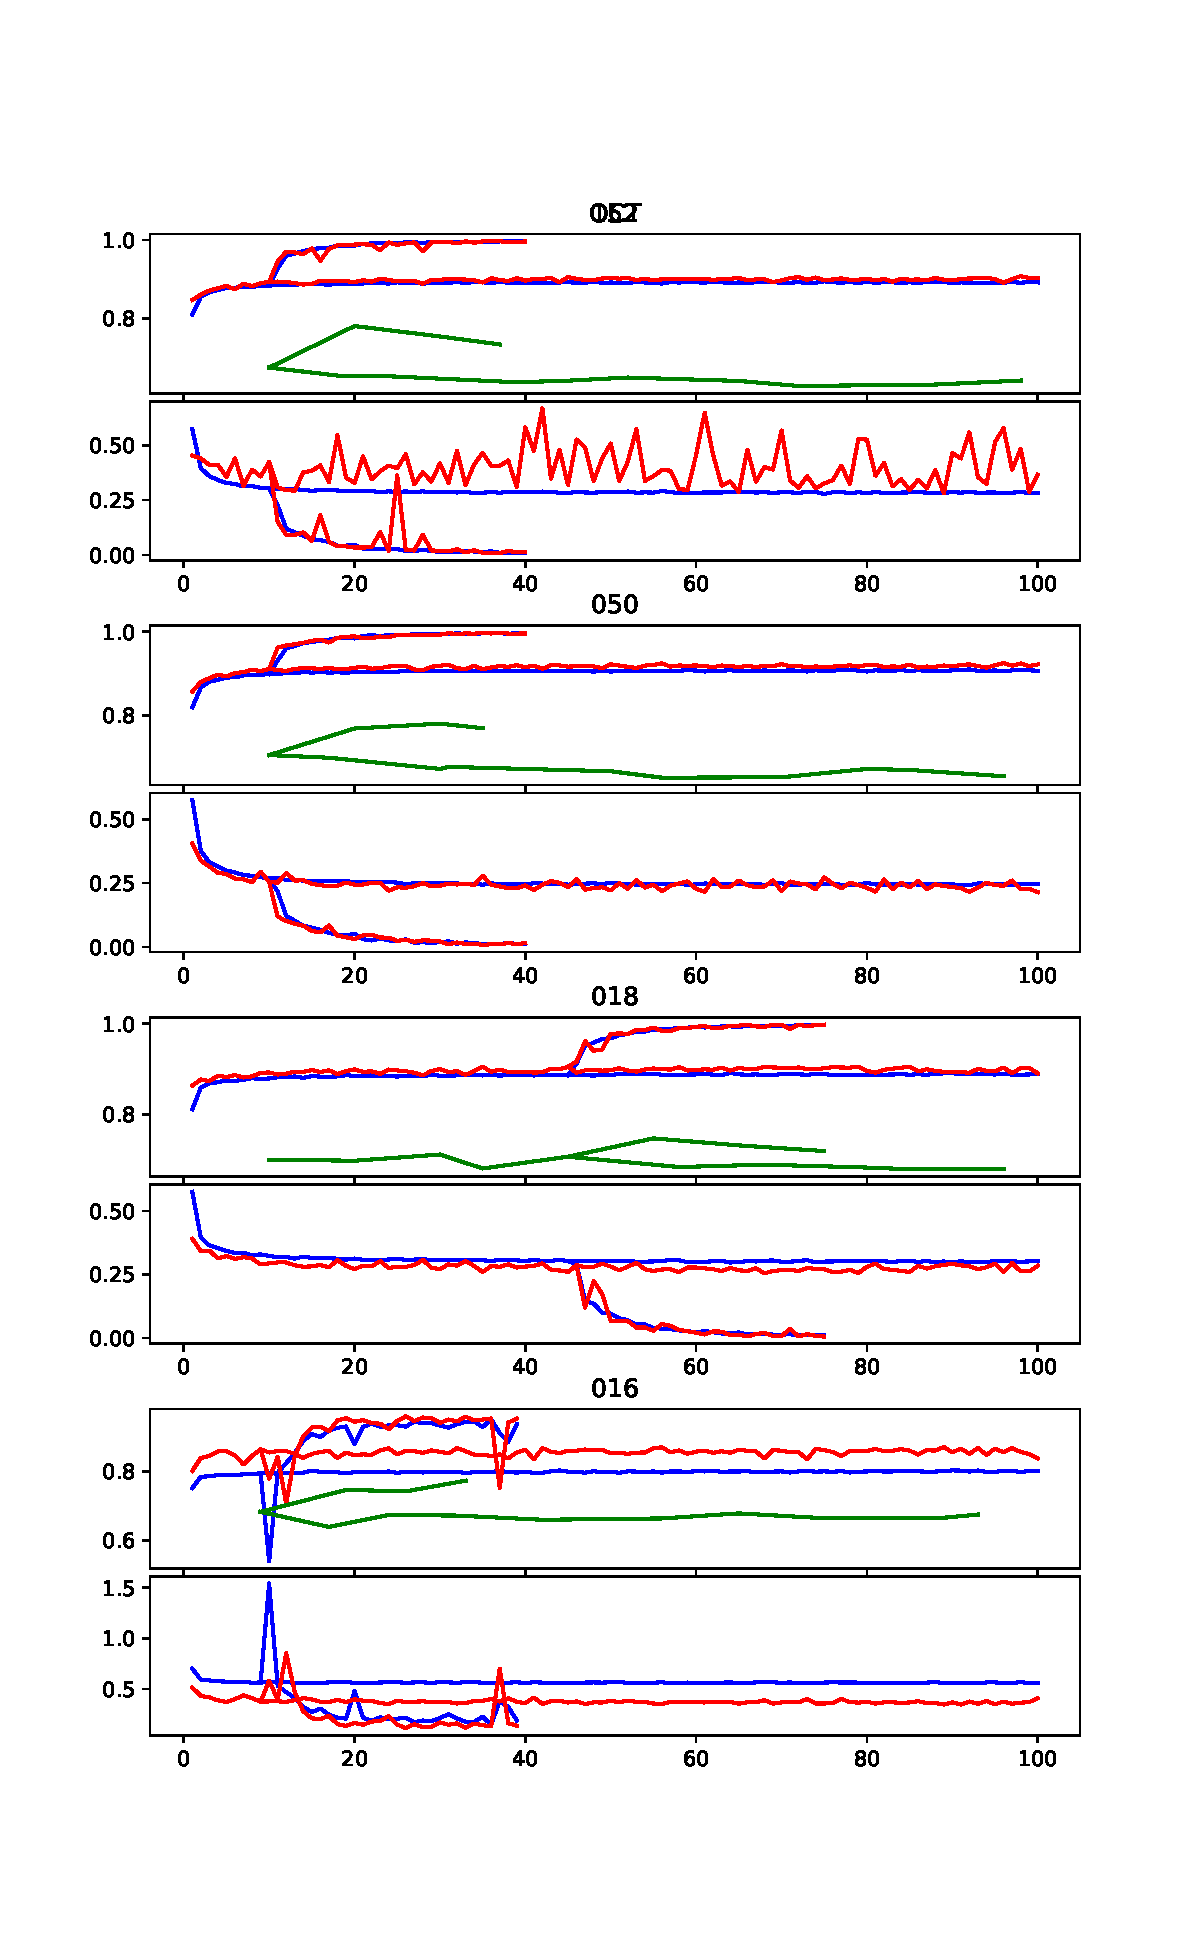
\includegraphics[width=\linewidth]{Figs/abnormity_OCT_loss_and_acc.pdf}
	\end{figure}
	\begin{figure}[htbp]
		\centering
		\vspace{-1cm}
		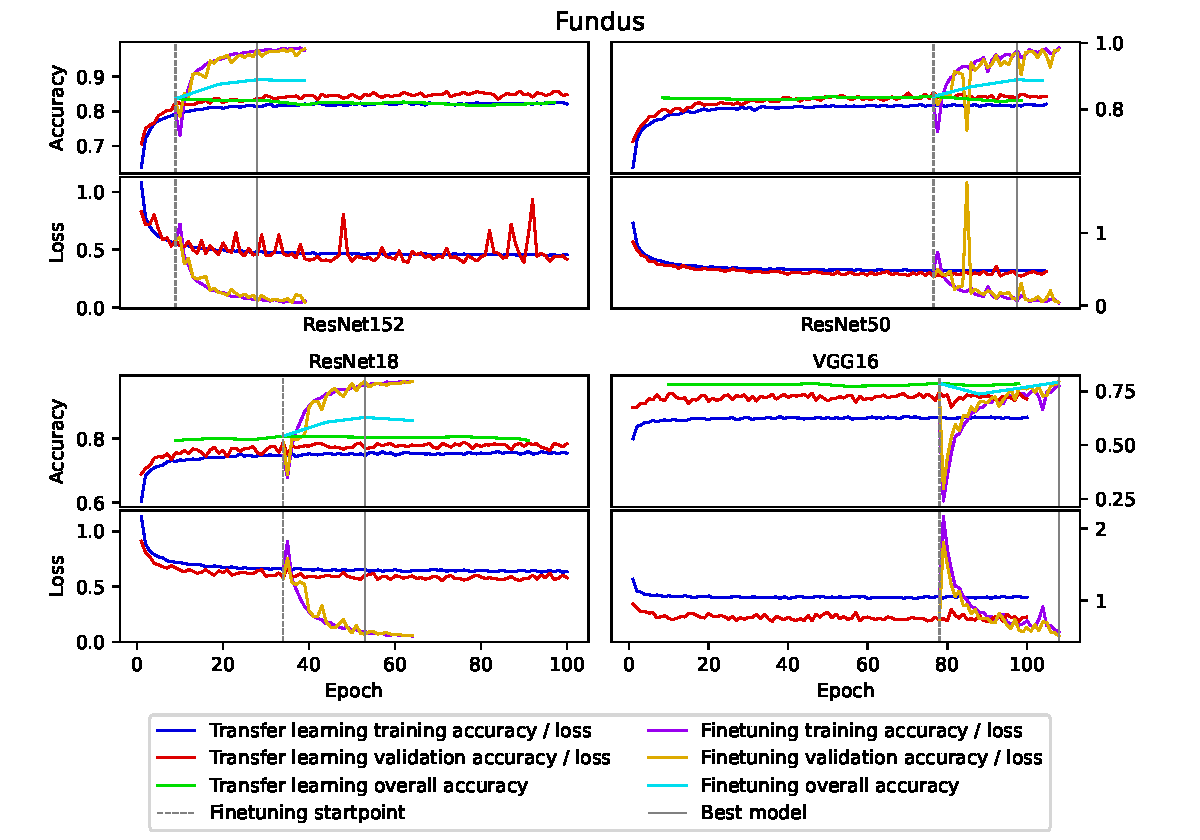
\includegraphics[width=\linewidth]{Figs/abnormity_Fundus_loss_and_acc.pdf}
		\caption{Abnormity training}
		\vspace{0.3cm}
		\label{fig:A_train}
	\end{figure}
		
	\pagebreak
	
	\vspace{0.3cm}
	
	We can observe that finetuning significantly increases the model accuracy and, therefore, all the final models are finetuned models. As shown in Table~\ref{tb:A_accuracies}, the best CNN for OCT Model is ResNet50 and the best for Fundus Model is ResNet152. ResNet50 performed better than ResNet152 on OCT, possibly because it has fewer parameters and is less likely to overfit on OCT images, which has fewer and clearer traits; on the other hand, ResNet152 is better on fundus possibly because it has more parameters and can better discern the complex traits in fundus images. ResNet18 may have too few parameters, so it performs less well over all; and VGG16 sometimes experiences large dips in accuracy, possibly due to gradient vanishing, and this impairs its performance. 
	
	\vspace{0.2cm}
	
	After all the training and comparisons, we determine to use a finetuned model with ResNet50 for OCT Model and a finetuned model with ResNet152 for Fundus Model. 
	
	{
		\fontsize{9}{12}\selectfont
		{
			\begin{table}
				\centering
				\caption{Overall accuracies}
				\label{tb:A_accuracies}
				\begin{tabular}{ccccc}
					\toprule
					Model&ResNet152&ResNet50&ResNet18&VGG16\\
					\midrule
					OCT Model   &91.906\%&\textbf{92.183\%}&91.011\%&89.744\% \\
					Fundus Model&\textbf{89.111\%}&88.926\%&86.605\%&79.185\% \\
					\bottomrule
				\end{tabular}
			\end{table}
		}
	}
	
	\subsection{Results}
	
	Table~\ref{tb:OCT_test} and Table~\ref{tb:Fundus_test} show the predictive values on the test dataset. Fig.~\ref{fig:A_ROC} shows the ROCs, Fig.~\ref{fig:A_conf_mat} shows the confusion matrices and Fig.~\ref{fig:A_tSNE} shows the t-SNE graphs for each abnormity.
	
	The OCT Model tends to overfit, while the Fundus Model cannot reach a satisfying level in terms of DL. Overall, the performance of the OCT Model is significantly better than that of the Fundus Model.
	
	Fundus abnormities tend to be less prominent than those of OCT, since the abnormity in fundus image are usually quite small and scattered. Moreover, one fundus image usually contains more than one abnormity, while most OCT images contain only one abnormity per image. Also, given that we have fewer fundus images than OCT ones, the difficulties for fundus classification increases.
	
	In order to allow the Abnormity Models to identify multiple abnormities in one image, we employ a method to determine the codominant abnormities. We input an image to the Abnormity Models and get the abnormity probabilities vector. If the abnormity with the highest probability has probability greater than 0.9, it is regarded as dominant; if not, we continue taking the abnormity with the next high probability until either the sum of the probabilities of the chosen abnormities reaches 0.9, or the number of abnormities reaches the maximum, which is 4, and all the chosen abnormities are regarded as codominant. 
	
			\begin{table}[htbp]
				\centering
				\fontsize{9}{12}\selectfont{
				\caption{OCT Test}
				\label{tb:OCT_test}
				\pgfplotstabletypeset[
				multicolumn names,
				col sep=comma,
				columns = {Abnormity, Precision, Sensitivity, Specificity, FOne, AUC},
				columns/Abnormity/.style={string type, column name=Abnormities},
				columns/Precision/.style={string type, column name=Precision},
				columns/Sensitivity/.style={string type, column name=Sensitivity},
				columns/Specificity/.style={string type, column name=Specificity},
				columns/FOne/.style={string type, column name={F1 Score}},
				columns/AUC/.style={string type, column name=AUC},
				every head row/.style={before row=\toprule, after row=\midrule},
				every last row/.style={ after row=\bottomrule}
				]{Tables/abnormity_o_test.csv}}
			\end{table}
	
			\begin{table}[htbp]
				\centering
				\fontsize{9}{12}\selectfont{
				\caption{Fundus Test}
				\label{tb:Fundus_test}
				\pgfplotstabletypeset[
				multicolumn names,
				col sep=comma,
				columns = {Abnormity, Precision, Sensitivity, Specificity, FOne, AUC},
				columns/Abnormity/.style={string type, column name=Abnormities},
				columns/Precision/.style={string type, column name=Precision},
				columns/Sensitivity/.style={string type, column name=Sensitivity},
				columns/Specificity/.style={string type, column name=Specificity},
				columns/FOne/.style={string type, column name={F1 Score}},
				columns/AUC/.style={string type, column name=AUC},
				every head row/.style={before row=\toprule, after row=\midrule},
				every last row/.style={after row=\bottomrule}
				]{Tables/abnormity_f_test.csv}}
			\end{table}

	\begin{figure}[htbp]
		\centering
		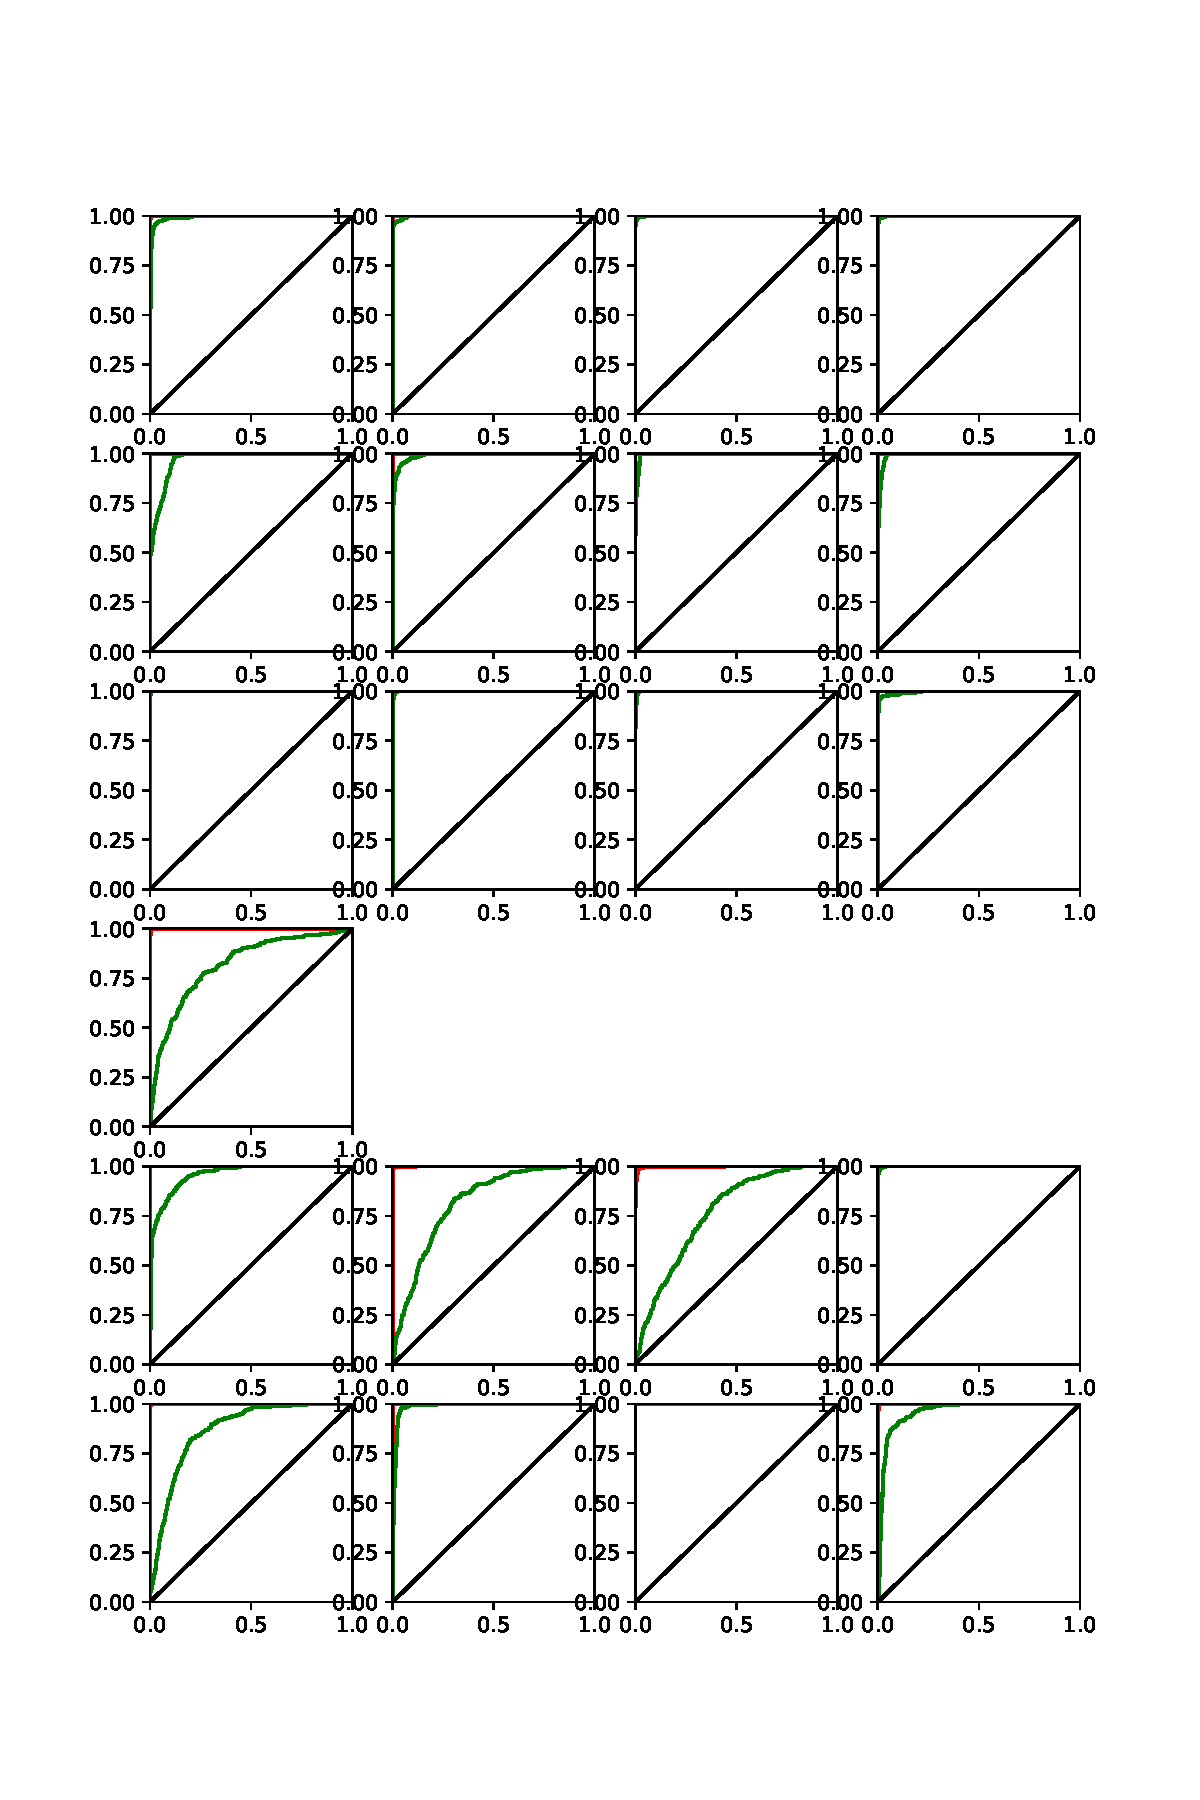
\includegraphics[width=\linewidth]{Figs/abnormity_ROC.pdf}
		\vspace{-1.5cm}
		\caption{A ROC}
		\vspace{0.3cm}
		\label{fig:A_ROC}
	\end{figure}
	
	\begin{figure}[htbp]
		\centering
		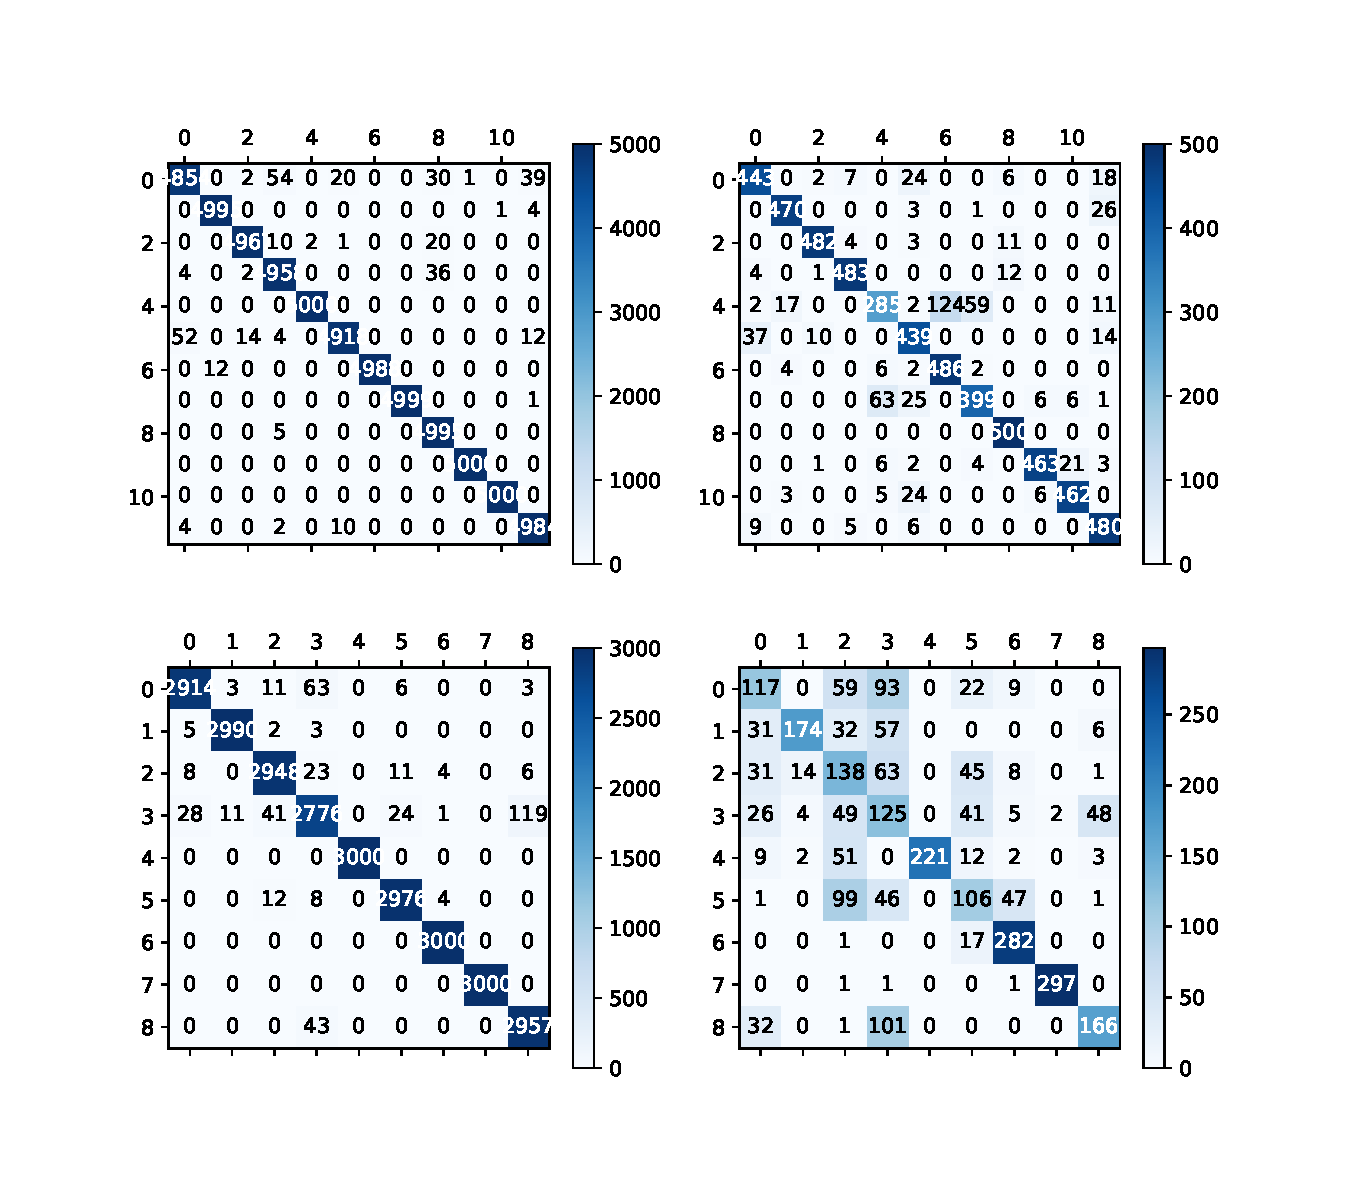
\includegraphics[width=\linewidth]{Figs/abnormity_confusion_matrix.pdf}
		\caption{A Conf Mat}
		\vspace{0.3cm}
		\label{fig:A_conf_mat}
	\end{figure}
	
	\begin{figure}[htbp]
		\centering
		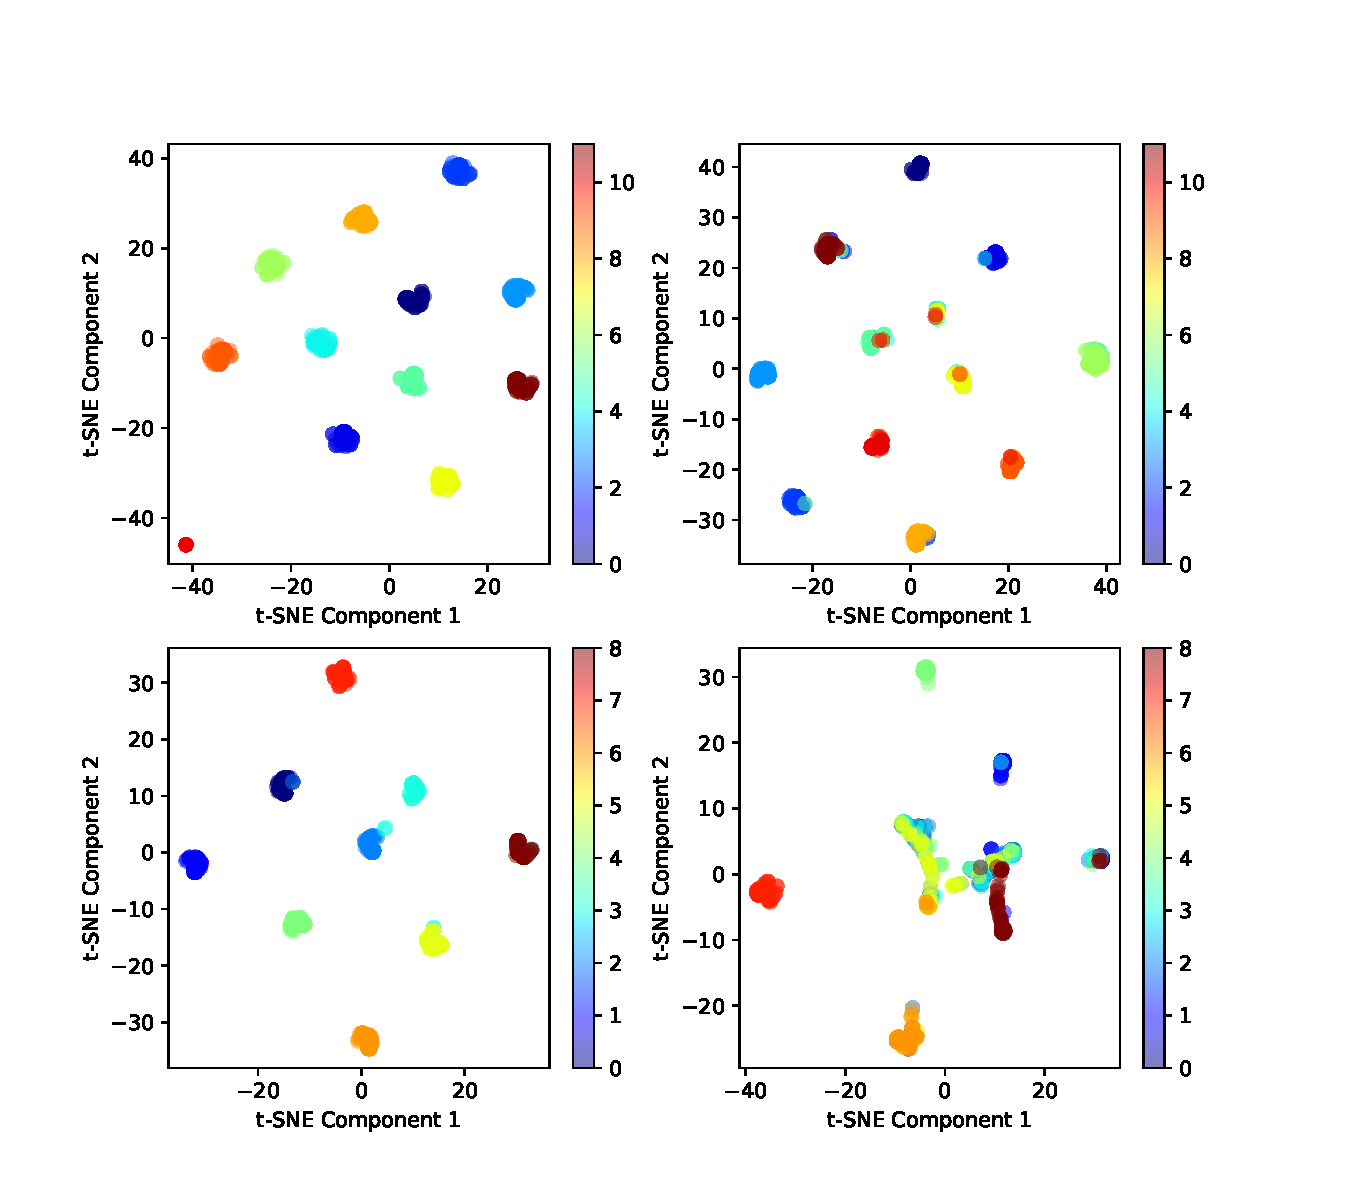
\includegraphics[width=\linewidth]{Figs/abnormity_tSNE.pdf}
		\caption{A ROC}
		\vspace{0.3cm}
		\label{fig:A_tSNE}
	\end{figure}
	
	\vspace{0.3cm}
	
	We can use Grad-CAM \autocite{Selvaraju_Cogswell_Das_Vedantam_Parikh_Batra} to highlight areas on the image that make a large contribution to the final classification. If the model had been trained correctly, this would be equivalent to highlighting the abnormity. In Fig.~\ref{fig:gradCAM}, the left image in each pair of images is the original OCT or Fundus image, and the right one is the image with the abnormity correctly highlighted with Grad-CAM. 
	
	Furthermore, Grad-CAM can highlight any designated abnormity, so it can be used to highlight codominant abnormities. In Fig.~\ref{fig:gradCAM_multi_abnormity}, the middle images are the original OCT and fundus images. In the images on the left and right, we use Grad-CAM to highlight the codominant abnormities.
	
	\begin{figure}[htbp]
		\centering
		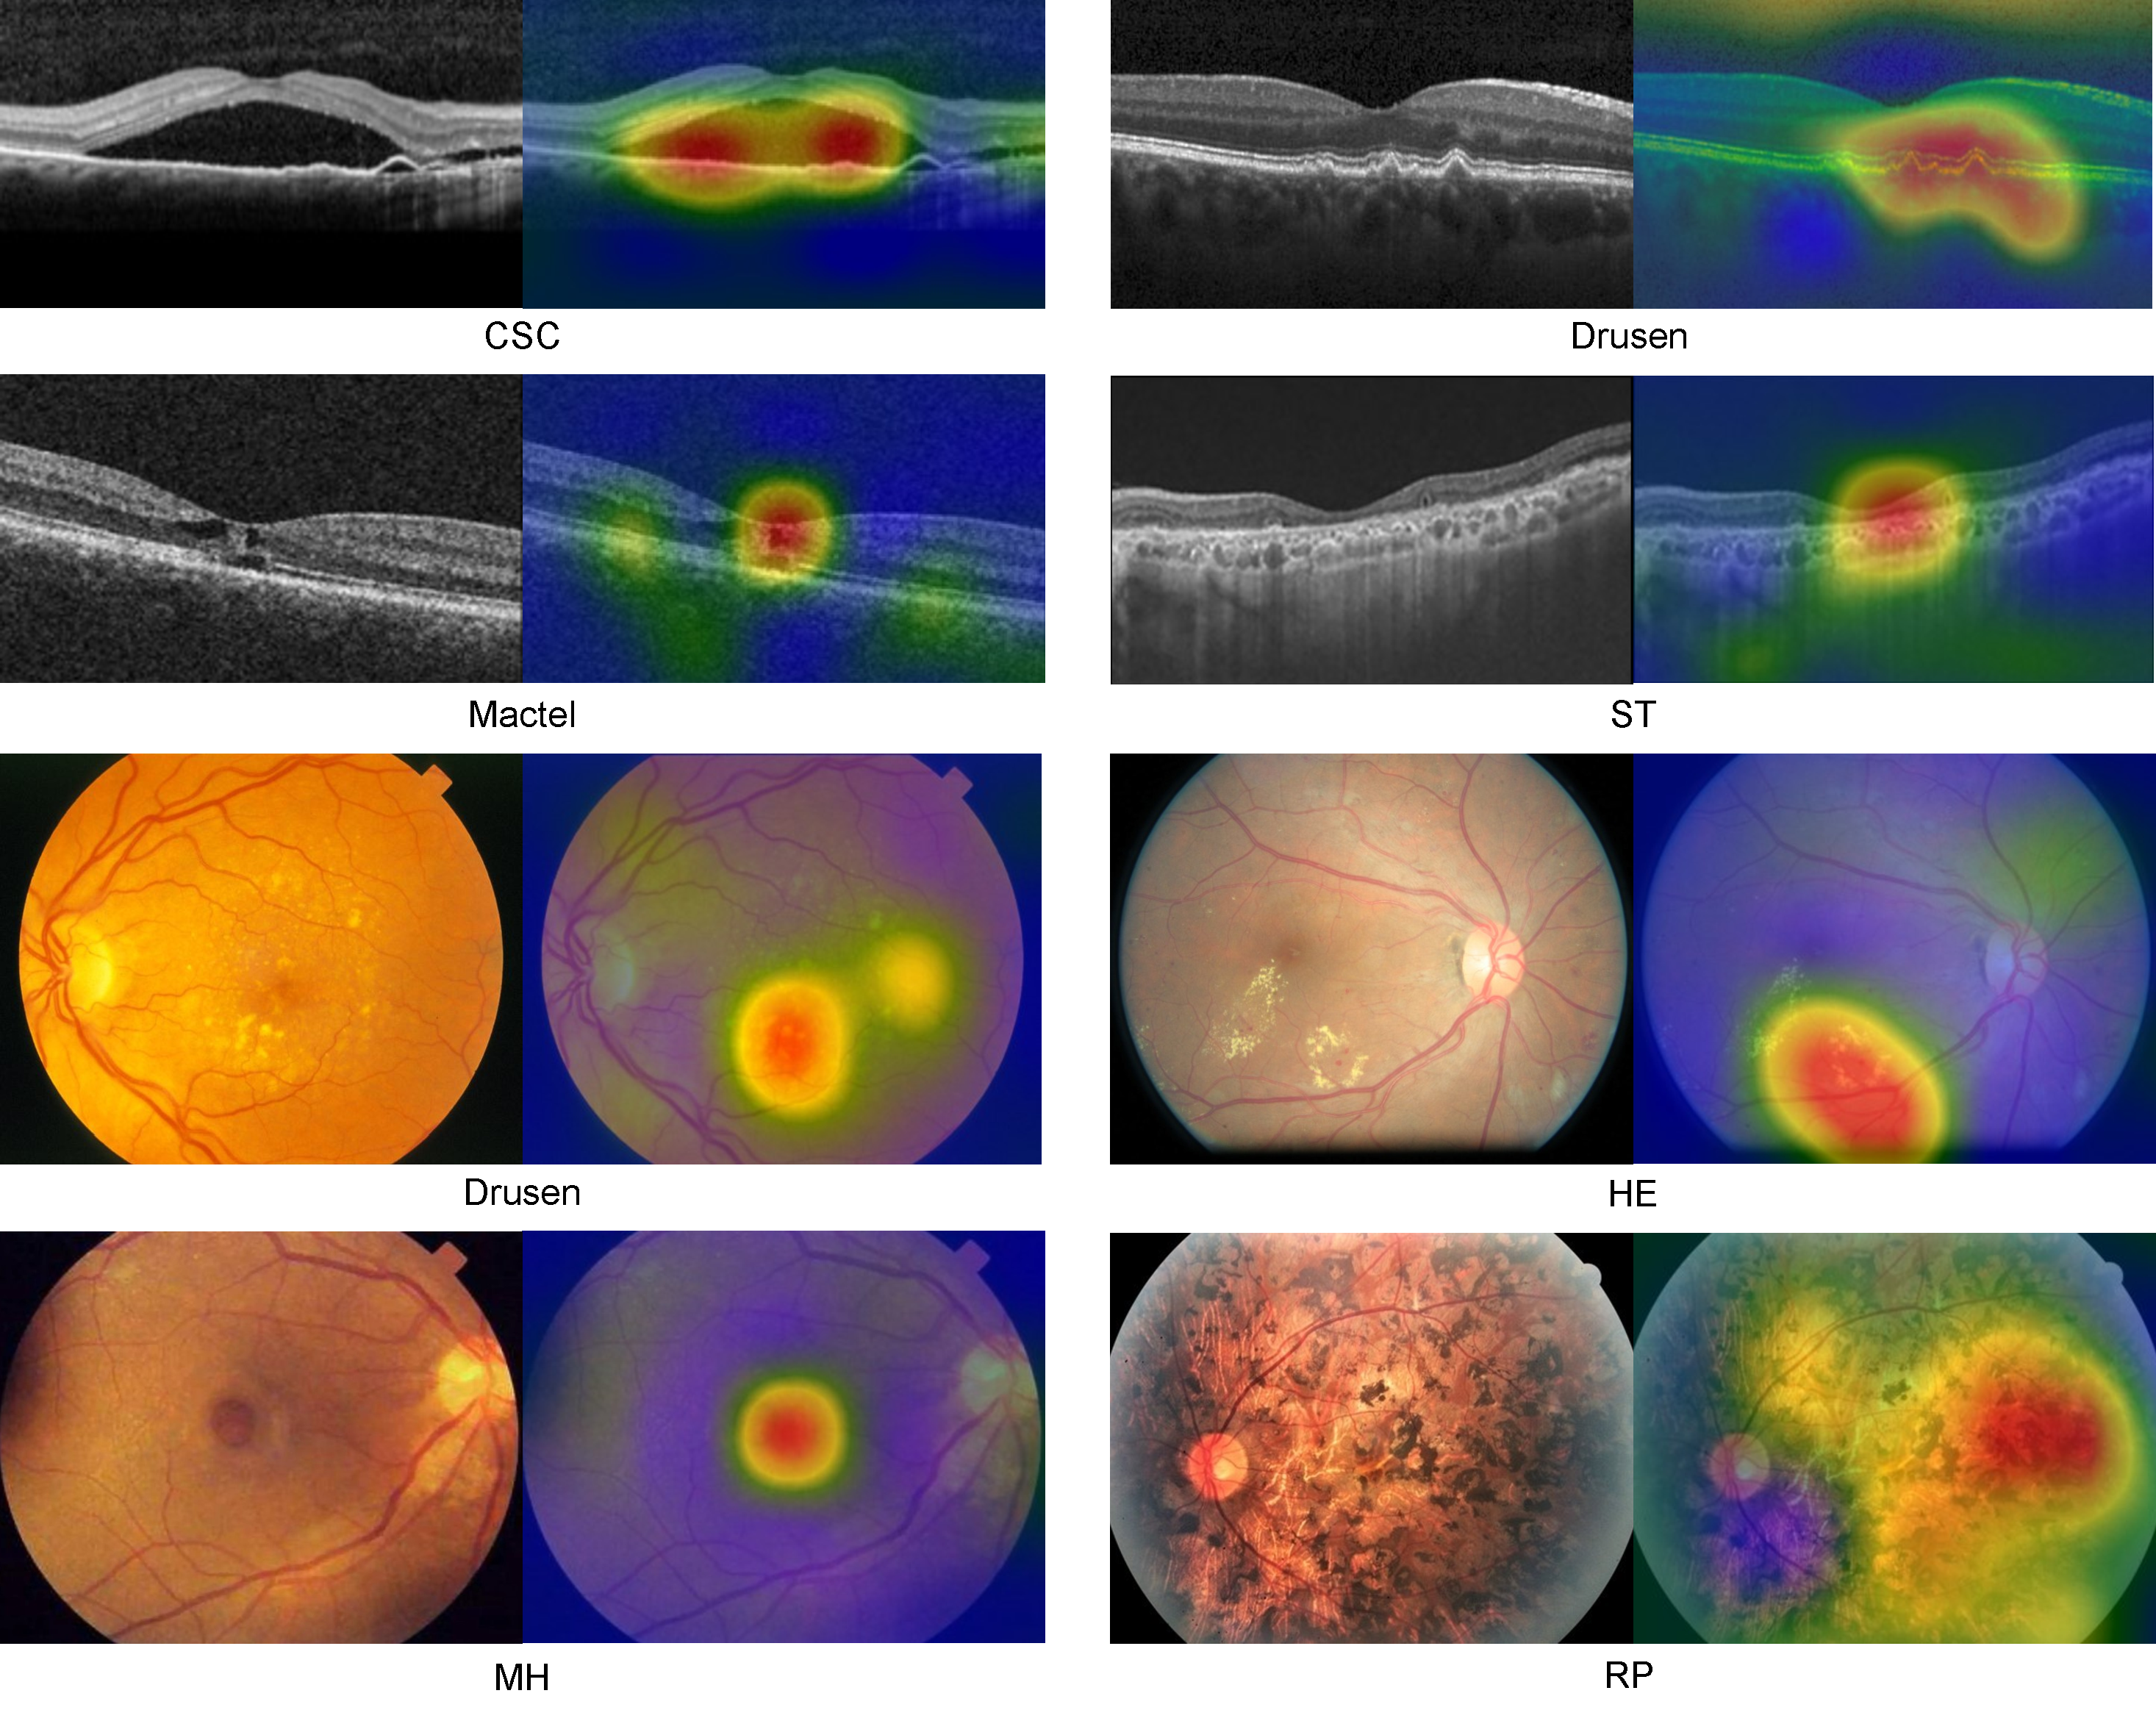
\includegraphics[width=\linewidth]{Figs/abnormity_gradCAM.pdf}
		\caption{GradCAM}
		\vspace{0.3cm}
		\label{fig:gradCAM}
	\end{figure}
	
	\begin{figure}[htbp]
		\centering
		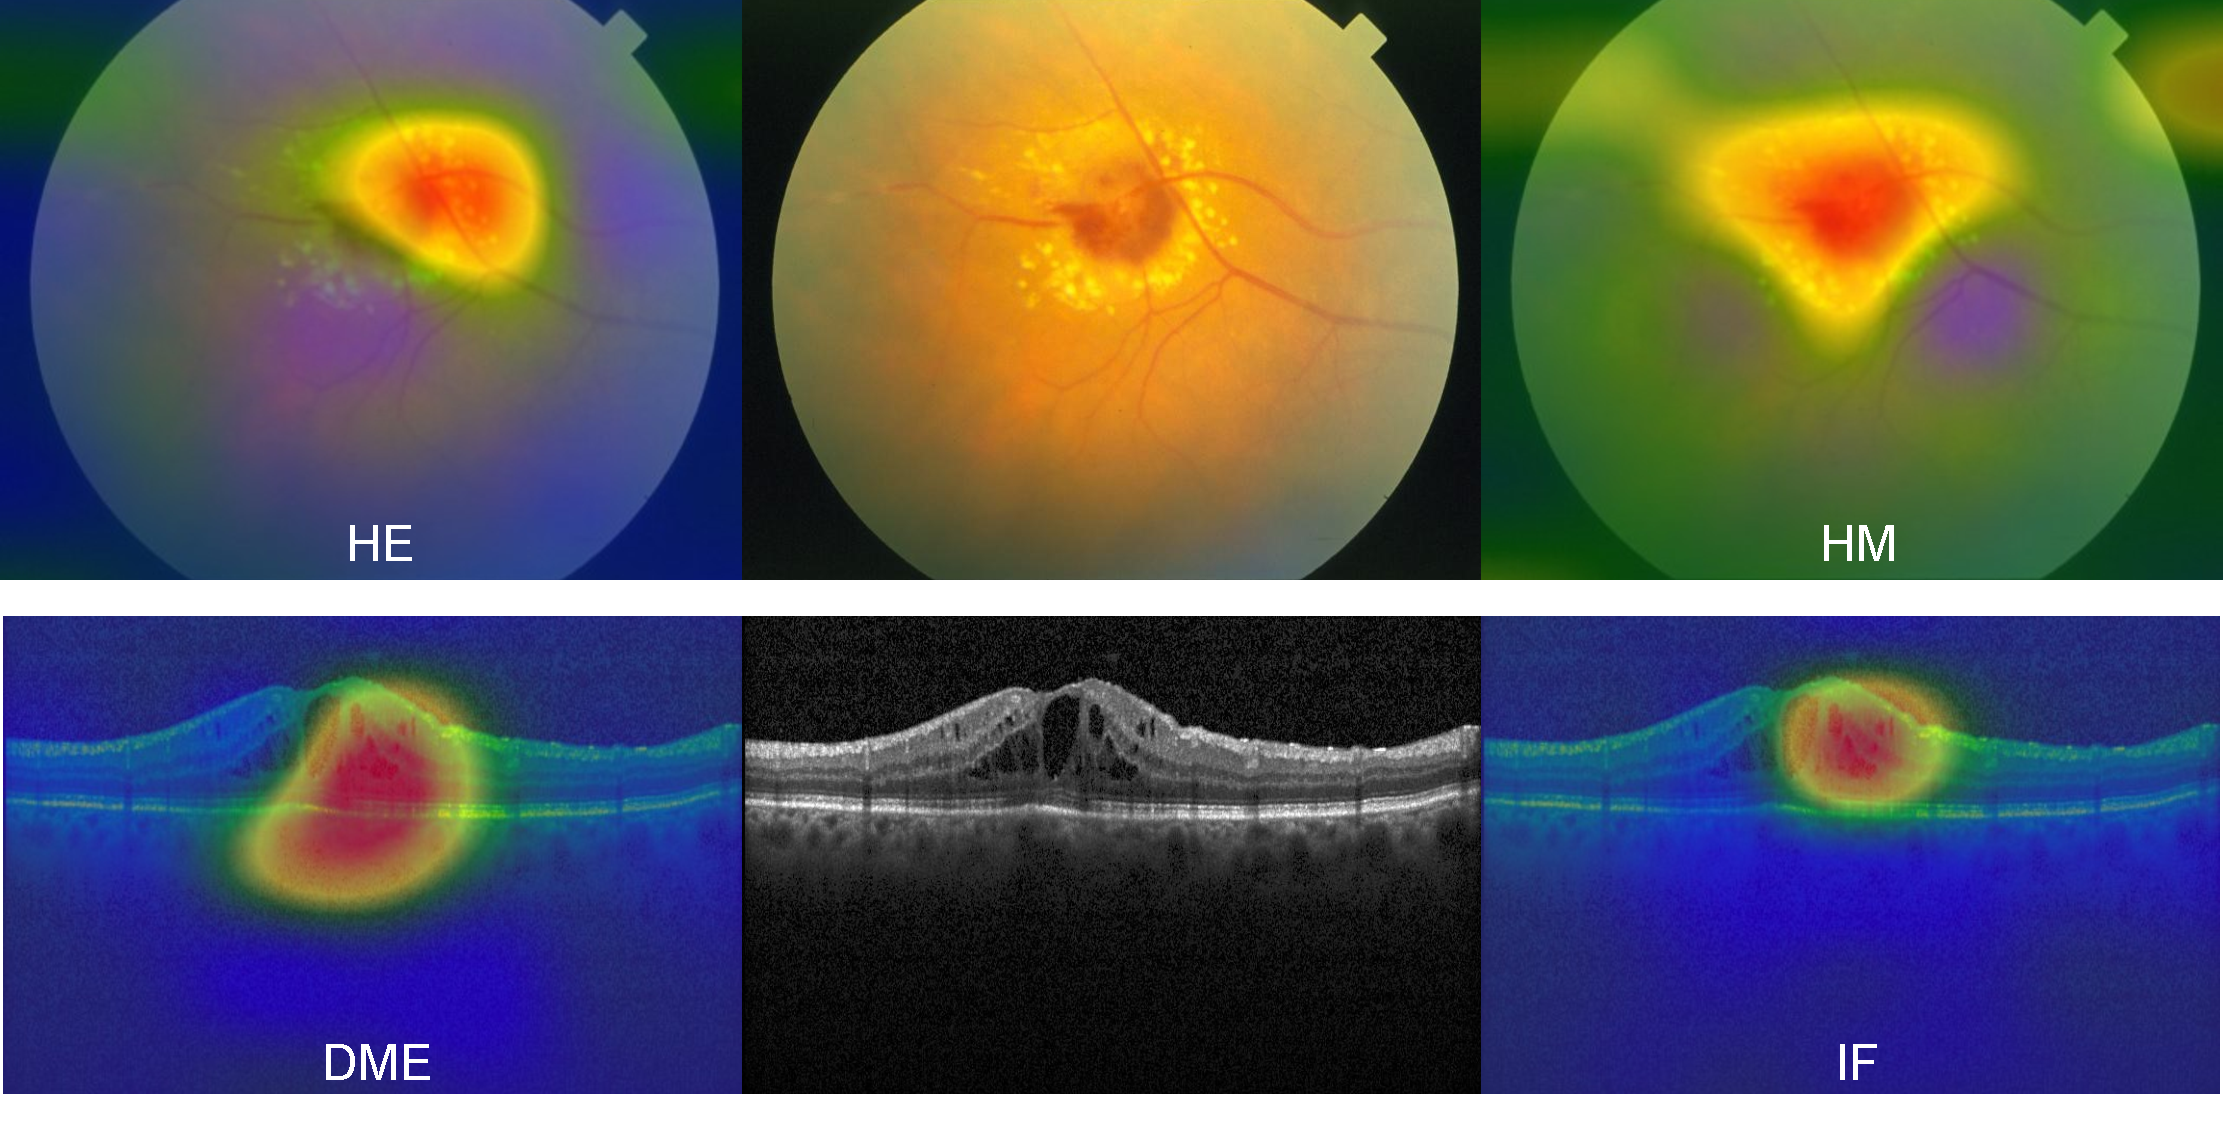
\includegraphics[width=0.8\linewidth]{Figs/abnormity_gradCAM_multiple_abnormities.pdf}
		\caption{GradCAM with multiple abnormities}
		\vspace{0.3cm}
		\label{fig:gradCAM_multi_abnormity}
	\end{figure}
	
	\section{Diagnosis Model}
	
	\subsection{Data Preparation}
	
	The purpose of Stage D1 is to determine the severity level for all diseases, each of which has a corresponding submodel. We prepare data for each submodel according to the Abnormity-to-Disease Deduction Criteria (shown in Fig.~\ref{fig:criteria}). As stated in Section~\ref{sec:overview}, we determine the target abnormities for one disease and use the number of target abnormities to define the severity levels. If a disease has 5 target abnormities, then, taking into account the healthy status, we get 6 severity levels, namely 0 to 5. We use sets of images as inputs to the submodel, and the severity level label for one set is equal to the number of target abnormities that appear in the set. We randomly choose sets of images from the OCT and fundus images and determine the severity level for each set. In the end, we get 10000 inputs for training and 10000 inputs for testing for each severity level. 
	
	The purpose of Stage D2 is to output the disease probability vectors. For each disease, we use the Abnormity-to-Disease Deduction Criteria to find the target abnormities, randomly choose sets of images where each of them is from one target abnormitiy, and label the sets of images with the disease. We get 10000 sets of images for training and 10000 sets of images for testing for each of the disease.
	
	\subsection{Training}
	
	The Diagnosis Model is trained with the same hardware as the Abnormity Models. Stage D1 submodels are trained for 10 epochs and Stage D2 model is trained for 30 epochs, and all the other hyperparameters are identical to those of the Abnormity Models. Refer to Section~\ref{sec:a_training} for details. 
	
	Submodels in Stage D1 and the model in Stage D2 quickly reach very high accuracies during training and validation because there are plenty of training data and the models leverage relatively simpler networks. 
	
	
	\subsection{Results}
	
	Fig.~\ref{fig:D1_conf_mat} shows the confusion matrices for Stage D1 and Fig.~\ref{fig:D1_acc_bar} shows the accuracies of the submodels of Stage D1. Table~\ref{tb:diagnosis_test} shows the predictive values of Stage D2, Fig.~\ref{fig:D2_ROC} shows the ROCs, Fig.~\ref{fig:D2_conf_mat} shows the confusion matrix and Fig~\ref{fig:D2_tSNE} shows the t-SNE graph.
	
	The submodels of Stage D1 tend to yield results where the predicted severity level is 1 level offset from the label. This impairs the accuracies of the submodels of Stage D1. However, Stage D2 partly solves this problem, as the model in Stage D2 has a higher accuracy than the average accuracy of the Stage D1 submodels. 
	
	Stage D2 performs quite well on classifying the diseases. Furthermore, considering that some diseases may look alike each other, we employ a method similar to the codominant abnormities method to allow Stage D2 to give up to 3 codominant diseases. As shown in Fig.~\ref{fig:D1_acc_bar}, if the codominant diseases method is used, the accuracy of Stage D2 further increases. 
	
	\begin{figure}[htbp]
		\centering
		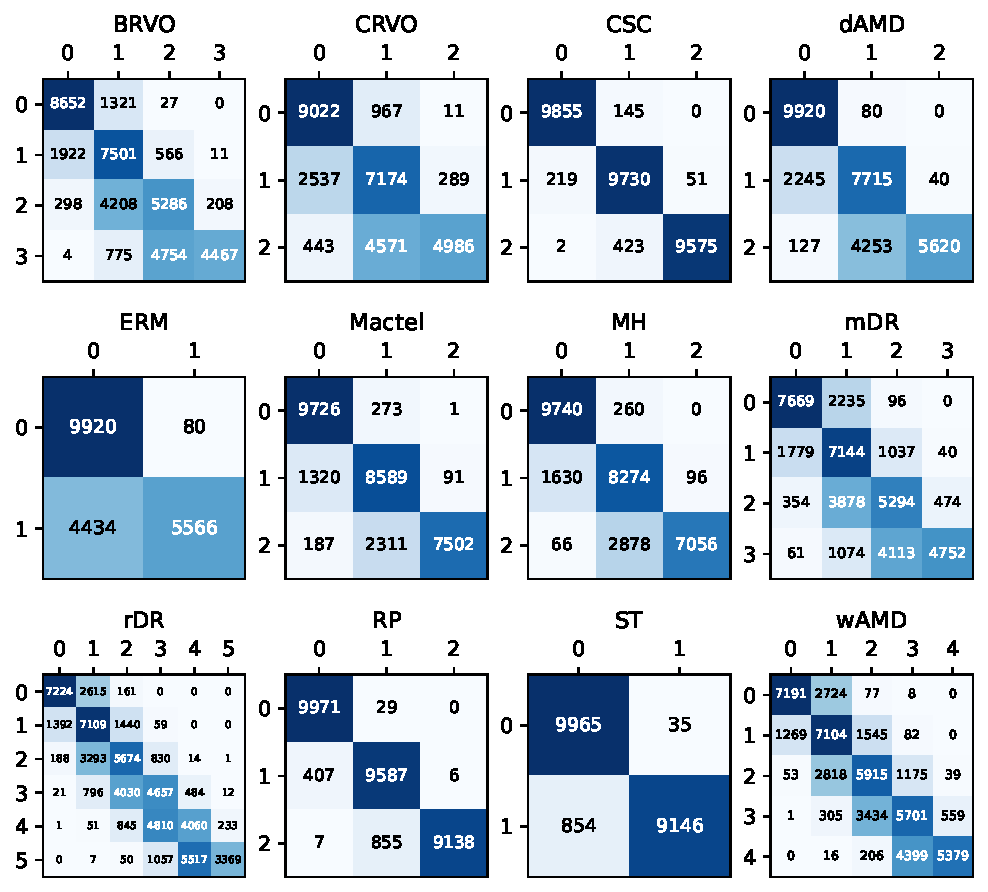
\includegraphics[width=\linewidth]{Figs/diagnosis1_confusion_matrix.pdf}
		\caption{D1 Conf Mat}
		\vspace{0.3cm}
		\label{fig:D1_conf_mat}
	\end{figure}
	
	\begin{figure}[htbp]
		\centering
		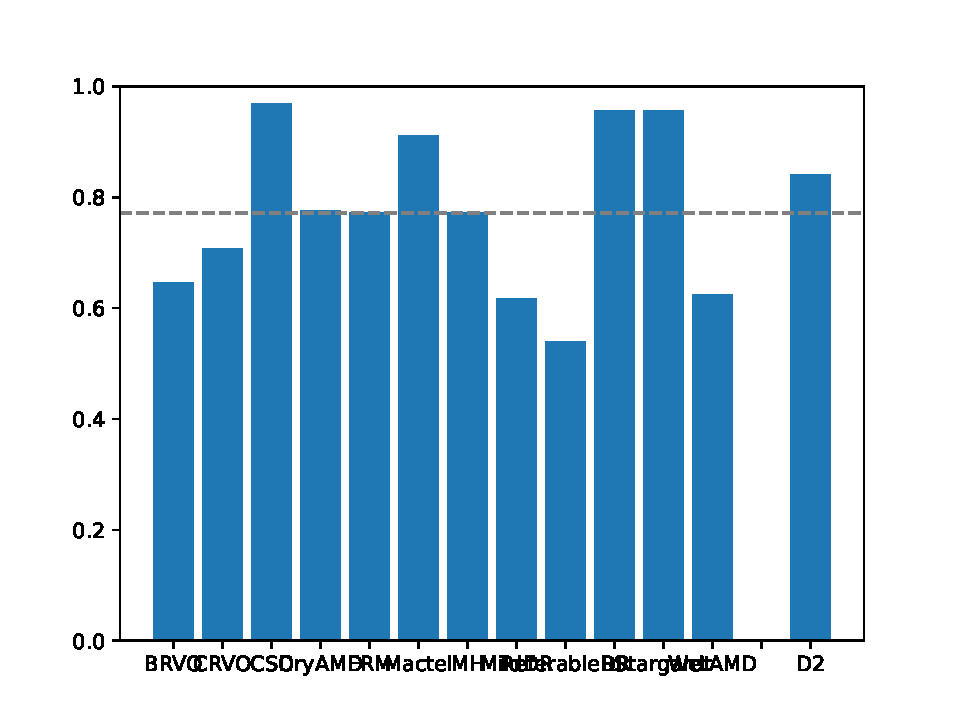
\includegraphics[width=\linewidth]{Figs/diagnosis1_acc_barchart.pdf}
		\caption{D1 Acc Bar}
		\vspace{0.3cm}
		\label{fig:D1_acc_bar}
	\end{figure}
	
	\begin{table}[htbp]
		\centering
		\fontsize{9}{12}\selectfont{
		\caption{Diagnosis Test}
		\label{tb:diagnosis_test}
		\pgfplotstabletypeset[
		multicolumn names,
		col sep=comma,
		columns = {Abnormity, Precision, Sensitivity, Specificity, FOne, AUC},
		columns/Abnormity/.style={string type, column name=Abnormities},
		columns/Precision/.style={string type, column name=Precision},
		columns/Sensitivity/.style={string type, column name=Sensitivity},
		columns/Specificity/.style={string type, column name=Specificity},
		columns/FOne/.style={string type, column name={F1 Score}},
		columns/AUC/.style={string type, column name=AUC},
		every head row/.style={before row=\toprule, after row=\midrule},
		every last row/.style={ after row=\bottomrule}
		]{Tables/diagnosis2.csv}}
	\end{table}
	
	\begin{figure}[htbp]
		\centering
		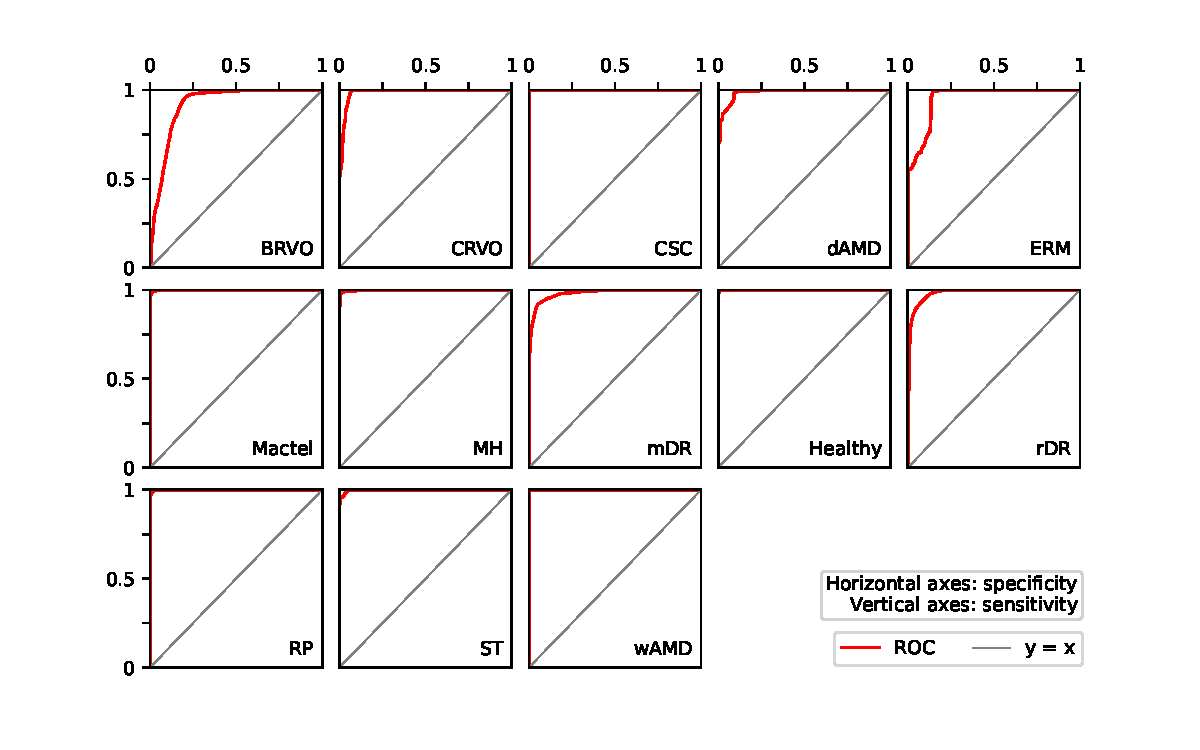
\includegraphics[width=\linewidth]{Figs/diagnosis2_ROC.pdf}
		\caption{D2 ROC}
		\vspace{0.3cm}
		\label{fig:D2_ROC}
	\end{figure}
	
	\begin{figure}[htbp]
		\centering
		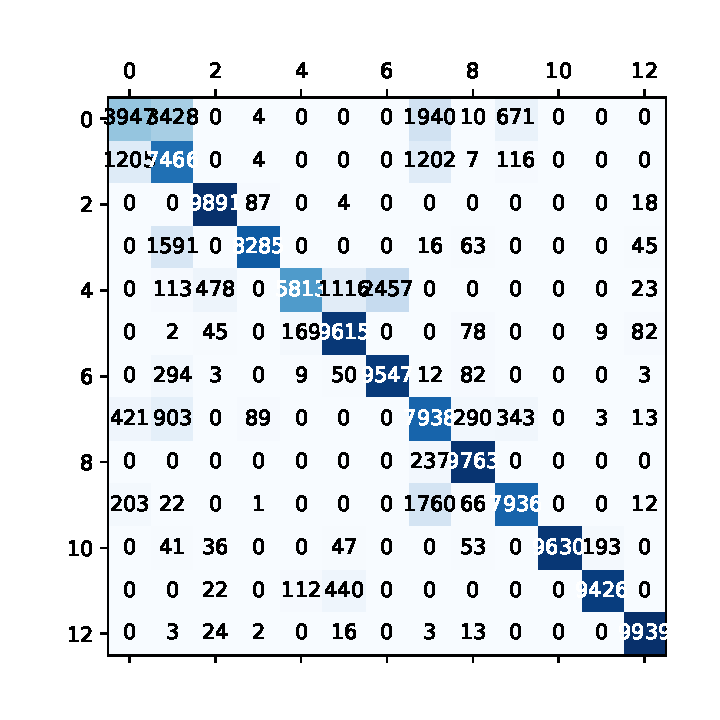
\includegraphics[width=\linewidth]{Figs/diagnosis2_confusion_matrix.pdf}
		\caption{D2 Conf Mat}
		\vspace{0.3cm}
		\label{fig:D2_conf_mat}
	\end{figure}
	
	\begin{figure}[htbp]
		\centering
		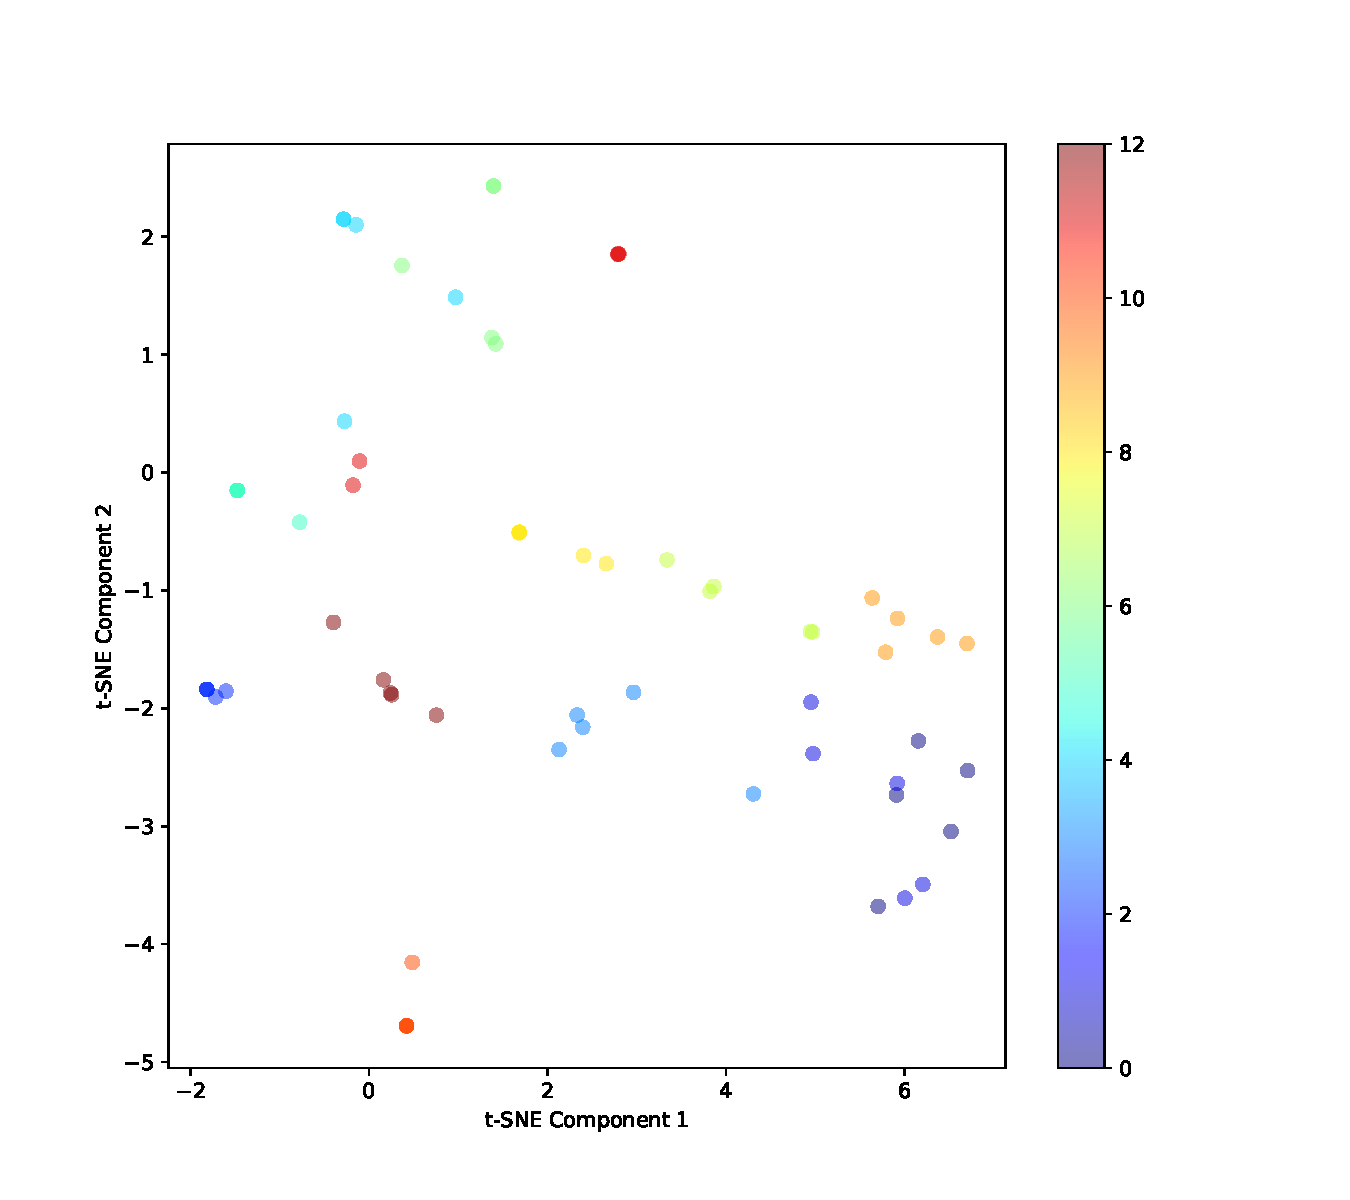
\includegraphics[width=\linewidth]{Figs/diagnosis2_tSNE.pdf}
		\caption{D2 tSNE}
		\vspace{0.3cm}
		\label{fig:D2_tSNE}
	\end{figure}
	
	\section{Discussion}
	
	There are some studies working on classifying OCT abnormities.  For examples, \citeauthor{leandro2023oct}'s model is trained on 10770 images (most images belong to multiple classes), classifies 8 abnormities, and has overall accuracy between 93\% and 99\% \autocite{leandro2023oct}. \citeauthor{li2019deep}'s model is trained on 21357 images, classifies 4 abnormities, and has overall accuracy 97.3\% \autocite{li2019deep}.  And there are some studies working on classifying fundus abnormities.  For example,  	\citeauthor{Son2023}'s model is trained on 103262 images, classifies 15 abnormities, and has a mean AUC of 0.980 \autocite{Son2023}. In comparison, our OCT Model is trained on 15632 images, classifies 11 abnormities, and has overall accuracy less than 80\%.  And our Fundus Model is trained on 1734 images, classifies 8 abnormities, and has a mean AUC of 0.909. As a matter of fact, our Abnormity Models are not satisfying in terms of performance.
	
	Our data are collected from various online sources and therefore lack a uniform standard. Furthermore, some of the data are labeled by ourselves, while we do not have the expertise of ophthalmologists. Moreover, our data is not sufficient. There is also an imbalance between the number of images of different abnormities. In the OCT Model, the imbalance is partly neutralized by using Cycle-GAN. However, in the Fundus Model, we could only perform transformations to generate more images, which may increase the model's tendency of being overfitting and make it hard for the model to extract the correct features. Also as mentioned before, in our model, there are often multiple abnormities on one image, which increase the difficulty to identify one specific abnormity correctly. 
	
	\vspace{0.3cm}
	
	In MAAM, the Diagnosis Model improves the overall performance successfully. There are also some studies using similar framework. For example, \citeauthor{Son2023}'s diagnosis model classifies 8 diseases and has mean AUC 0.992\autocite{Son2023}. In comparison, our Diagnosis Model classifies 12 diseases and has mean AUC of 0.984 which is close to other studies.
	
	It is noted that the goal of MAAM is not to identify one specific disease.  It is developed for identifying all the potential diseases, which is different from other studies mentioned in this paper.  Therefore, we introduced codominant abnormities and codominant diseases, which buff up the performances. Moreover, the Diagnosis Model performs two additional feature extractions. While the Abnormity Models only have accuracies between 70\% and 80\%, after we extracted the features of severity levels of diseases in Stage D1, the average accuracy increases. And after we extracted the features of disease in Stage D2, the accuracy keep on increasing up to a satisfying level. These two stages enhance the performance of the Abnormity Models and make the features of the diseases more distinct.	Also, in training the Diagnosis Model, we use the Abnormity-to-Disease Deduction Criteria to generate ground truth, which is reliable even without involving ophthalmologists.
	
	\section{Conclusion}
	
	The main goal of this study is to devise a novel model and verify its feasibility. The MAAM takes both OCT and fundus images as input. We integrate information from different sources by employing the fusion mechanism. Moreover, we deduce disease from abnormities and simulate the decision-making process of ophthalmologists. We also introduced codominant abnormities and diseases, providing more information for reference. As a result, the model breaks the black box of complex neural network and exposes more information. On the other hand, there is some room for improvement, such as gathering more authentic data, introducing the expertise of ophthalmologists, refining the Abnormity-to-Disease Deduction Criteria, and improving the structure of the Diagnosis Model, etc.
	
	\phantomsection
	\addcontentsline{toc}{section}{References}
	\newrefcontext[sorting=nyt]
	\printbibliography
	
	\pagebreak
	\section*{Appendix}
	
	\subsection*{Code}
	
	The link for the GitHub repository is \url{https://github.com/SiqiPan2008/MAAM/}.
	
	\subsection*{Abnormities and Diseases}
	
	{
		\fontsize{9}{12}\selectfont
		{
			\begin{longtable}{llp{9.5cm}}
				\caption*{OCT Abnormities}
				\label{tb:oct-abnormites}\\
				\toprule
				Abnormity&Abbr.&Description\\
				\toprule
				
				Choroidal neovascularization
				& CNV
				& The abnormal growth of new blood vessels in the choroid layer.\\
				
				Central serous chorioretinopathy
				& CSC
				& The accumulation of fluid underneath the retina.\\
				
				Diabetic macular edema
				& DME
				& The accumulation of fluid in the macula associated with diabetic retinopathy. \\
				
				Drusen
				& Drusen
				& Small deposits of extracellular material that accumulate beneath the retinal pigment epithelium (RPE) or between the RPE and the photoreceptor layer in the macular region of the retina.\\
				
				Epiretinal membrane
				& ERM
				& A thin layer of fibrous tissue forms on the surface of the retina, particularly the macula.\\
				
				Intraretinal fluid
				& IF
				& The accumulation of fluid within the layers of the retina.\\
				
				Macular hole
				& MH
				& Disruption or discontinuity in the normal retinal layers surrounding the macular hole.\\
				
				Macular telangiectasia
				& Mactel
				& Abnormities in the macular blood vessels, leading to changes in the macular structure and function.\\
				
				Retinitis pigmentosa
				& RP
				& Thinning of the retinal layers. Disruption of photoreceptor layers. Attenuation of retinal vasculature.\\
				
				Stargardt disease
				& ST
				& Thinning and atrophy of the retina. Disruption of photoreceptor layers. Presence of subretinal deposits.\\
				
				Subretinal fluid
				& SF
				& The accumulation of fluid between the neurosensory retina and the retinal pigment epithelium (RPE)\\
				
				\bottomrule
			\end{longtable}
		}
	}
	
	{
		\fontsize{9}{12}\selectfont
		{
			\begin{longtable}{llp{11.2cm}}
				\caption*{Fundus Abnormalities}
				\label{tb:fundus-ab}\\
				\toprule
				Abnormity&Abbr.&Description\\
				\toprule
				
				Cotton wool patch
				& CWP
				& White or off-white lesions. Irregular shapes and margins. Also called soft exudates. \\
				
				Drusen
				& Drusen
				& Small, round or oval-shaped yellow or white deposits.\\
				
				Hard exudate
				& HE
				& Yellow or Yellow-White Deposits. Hard Borders. Distribution. Clustering Around Blood Vessels\\
				
				Hemorrhage
				& HM
				& Small dot-like to larger blot. Fresh hemorrhages typically appear bright red or deep red in color, indicating the presence of oxygenated blood. Over time, as the blood undergoes degradation and clotting, the hemorrhage may change color to darker red, orange, or yellowish hues.\\
				
				Macular hole
				& MH
				& Full-thickness macular hole showing a surrounding cuff of subretinal fluid.\\
				
				Microaneurysm
				& MA
				& Small vascular dilatations observed in retinal blood vessels, visible as tiny red dots scattered in the retina posteriorly.\\

				Retinitis pigmentosa
				& RP
				& Arteriolar attenuation. Retinal pigmentary changes (either hypopigmentation and/or hyperpigmentation in the form of bone-spicule and pigment clumpings). Waxy disc pallor.\\

				Vascular abnormity
				& VA
				& Retinal Vessel Tortuosity. Retinal Vessel Caliber Changes. \\
				
				\bottomrule
			\end{longtable}
		}
	}
	
	{
		\fontsize{9}{12}\selectfont
		{
			\begin{longtable}{cc}
				\caption*{Diseases}
				\label{tb:diseases}\\
				\toprule
				Disease&Abbr.\\
				\toprule
				
				Branch or hemi-central retinal vein occlusion&BRVO\\
				Central retinal vein occlusion&CRVO\\
				Central serous chorioretinopathy&CSC\\
				Dry age-related macular degeneration&dAMD\\
				Epiretinal membrane&ERM\\
				Macular telangiectasia&Mactel\\
				Macular hole&MH\\
				Mild diabetic retinopathy&mDR\\
				Referable diabetic retinopathy&rDR\\
				Retinitis pigmentosa&RP\\
				Stargardt disease&ST\\
				Wet age-related macular degeneration&wAMD\\
				\bottomrule
			\end{longtable}
		}
	}
	
	\subsection*{Image Sources}
	
	\subsubsection*{OCT -- ERM}
	\vspace{0.5cm}
	
	\begin{enumerate}
		\item \nolinkurl{https://qers.com.au/eye-conditions/epiretinal-membrane-erm/}
		
		\item \nolinkurl{https://www.asrs.org/patients/retinal-diseases/19/epiretinal-membranes}
		
		\item \nolinkurl{https://theretinagroup.com/epiretinal-membrane/}
		
		\item \nolinkurl{https://www.istanbulretina.com/en-diseases-epiretinal-membrane.php}
		
		\item \nolinkurl{https://www.mdfoundation.com.au/about-macular-disease/other-macular-conditions/epiretinal-membrane-macular-pucker/}
		
		\item \nolinkurl{https://www.researchgate.net/figure/Grading-of-epiretinal-membrane-ERM-by-spectral-domain-optical-coherence-tomography_fig1_351426760}
		
		\item \nolinkurl{https://www.singhealth.com.sg/patient-care/conditions-treatments/epiretinal-membrane}
		
		\item \nolinkurl{https://www.windycityretina.com/epiretinal-membrane/}
		
		\item \nolinkurl{https://retinacentertx.com/conditions/macular-pucker}
		
		\item \nolinkurl{https://www.rvscny.com/patient-eduction/conditions-we-treat/epiretinal-membrane/}
		
		\item \nolinkurl{https://www.lyneye.co.za/epiretinal-membrane-erm/}
		
		\item \nolinkurl{https://rehmansiddiqui.com/epi-retinal-membrane-erm/}
		
		\item \nolinkurl{https://www.reviewofophthalmology.com/article/when-and-how-to-peel-an-epiretinal-membrane}
		
		\item \nolinkurl{https://www.janigianretina.com/retina-conditions/epiretinal-membrane}
		
		\item \nolinkurl{https://www.researchgate.net/figure/6-months-later-ERM-with-partial-attachment-to-the-retina_fig2_309566437}
		
		\item \nolinkurl{https://www.capefearretina.com/epiretinal-membrane/}
	\end{enumerate}
	
	\subsubsection*{Fundus -- MH}
	\vspace{0.5cm}
	
	\begin{enumerate}
			\item \nolinkurl{https://emedicine.medscape.com/article/1224320-overview}
			
			\item \nolinkurl{https://www.chatswoodeye.com/macular-hole-specialists/}
			
			\item \nolinkurl{https://swretina.com/macular-hole/}
			
			\item \nolinkurl{https://www.ophthalmologyexpertservices.com/blog/2019/macular-hole}
			
			\item \nolinkurl{https://www.researchgate.net/publication/38109568_Bilateral_macular_hole_secondary_to_remote_lightning_strike}
			
			\item \nolinkurl{https://www.researchgate.net/publication/38109568_Bilateral_macular_hole_secondary_to_remote_lightning_strike}
			
			\item \nolinkurl{https://www.reviewofoptometry.com/article/facedown-showdown}
			
			\item \nolinkurl{https://www.gotzaridis.gr/en/conditions/macula/full-thickness-macular-hole}
			
			\item \nolinkurl{https://www.researchgate.net/figure/Fundus-image-of-the-right-eye-of-case-1-a-shows-a-macular-hole-with-associated-retinal_fig1_324657341}
			
			\item \nolinkurl{https://www.girayersoz.com.tr/en/macular-hole/}
			
			\item \nolinkurl{https://www.gotzaridis.gr/en/conditions/macula/full-thickness-macular-hole}
			
			\item \nolinkurl{https://www.gotzaridis.gr/en/conhttps://www.willseye.org/macular-hole/ditions/macula/full-thickness-macular-hole}
			
			\item \nolinkurl{https://www.willseye.org/macular-hole/}
			
			\item \nolinkurl{http://www.oculist.net/downaton502/prof/ebook/duanes/pages/v3/ch031/013f.html}
			
			\item \nolinkurl{https://www.slideshare.net/slideshow/macular-hole-227845841/227845841#11}
			
			\item \nolinkurl{https://www.slideshare.net/slideshow/macular-hole-227845841/227845841#12}
			
			\item \nolinkurl{https://www.jaypeedigital.com/book/9788180616532/chapter/ch7}
			
			\item \nolinkurl{https://emedicine.medscape.com/article/1224320-clinical?form=fpf}
			
			\item \nolinkurl{https://www.jaafarelannanmd.com/macular-hole}
			
			\item \nolinkurl{https://asiaeyecentre.com.sg/eye-conditions/the-ageing-eye/macular-hole/}
			
			\item \nolinkurl{https://retinaandeye.com.au/eye-conditions/full-thickness-macular-holes/}
			
			\item \nolinkurl{https://retinahi.com/interesting-cases/}
			
			\item \nolinkurl{https://imagebank.asrs.org/file/2858/traumatic-macular-hole}
			
			\item \nolinkurl{https://www.semanticscholar.org/paper/Giant-macular-hole-as-an-atypical-consequence-of-a-Blaise-Comhaire/5c9a60375d904323eb5fbcd52b6bd03b735f6951}
			
			\item \nolinkurl{https://webeye.ophth.uiowa.edu/eyeforum/atlas/pages/Macular-hole-commotio-retinae-choroidal-rupture.htm#gsc.tab=0}
			
			
			\item \nolinkurl{https://areaoftalmologica.com/en/terms-of-ophthalmology/macular-hole/}
			
			\item \nolinkurl{https://www.reviewofoptometry.com/article/facedown-showdown}
			
			\item \nolinkurl{https://montanaretinaconsultants.com/portfolio/macular-holes/}
			
			\item \nolinkurl{https://ccteyes.com/2019/09/30/what-is-a-macular-hole-and-how-does-it-affect-your-vision/}
			
			\item \nolinkurl{https://www.backoftheeyemd.com/retina-services/macular-holes/}
			
			\item \nolinkurl{https://www.asrs.org/content/images/cms/image_rib_macularhole_2_2858.jpg/image-full;size$250,194.ImageHandler}
			
			\item \nolinkurl{https://www.asrs.org/content/images/cms/image_rib_macularhole_2_2858.jpg/image-full;size$250,194.ImageHandler}
			
			\item \nolinkurl{https://www.asrs.org/content/images/cms/image_rib_macularhole_2_2858.jpg/image-full;size$250,194.ImageHandler}
			
			\item \nolinkurl{https://webeye.ophth.uiowa.edu/eyeforum/atlas/pages/extrafoveal-macular-hole/emh-1.jpg}
	\end{enumerate}
	
	\subsubsection*{Fundus -- RP}
	\vspace{0.5cm}
		
	\begin{enumerate}
		\item \nolinkurl{https://imagebank.asrs.org/file/93471/retinitis-pigmentosa}
		
		\item \nolinkurl{https://educate.choroida.com/2021/07/05/retinitis-pigmentosa/}
		
		\item \nolinkurl{https://decisionmakerplus.net/dg-post/h35-52-retinitis-pigmentosa/}
		
		\item \nolinkurl{https://basicmedicalkey.com/retinitis-pigmentosa/}
		
		\item \nolinkurl{https://www.news-medical.net/health/What-is-Retinitis-Pigmentosa.aspx}
		
		\item \nolinkurl{https://www.researchgate.net/figure/Fundus-photograph-of-an-individual-affected-with-retinitis-pigmentosa-The-fundus_fig3_40447070}
		
		\item \nolinkurl{https://www.ncbi.nlm.nih.gov/books/NBK11553/figure/ch36clinicalerg.F15/}
		
		\item \nolinkurl{https://www.brainkart.com/article/Retinal-Dystrophies--Retinitis-Pigmentosa_26087/}
		
		\item \nolinkurl{https://entokey.com/retinitis-pigmentosa-and-allied-disorders/}
		
		\item \nolinkurl{https://entokey.com/retinitis-pigmentosa-and-allied-disorders/}
		
		\item \nolinkurl{https://retinography.org/sector-retinitis-pigmentosa/}
		
		\item \nolinkurl{https://retinography.org/sector-retinitis-pigmentosa/}
		
		\item \nolinkurl{https://www.linkedin.com/posts/stevenlevymd_blindness-from-retinitis-pigmentosa-reversed-activity-7047214648877608960-ar4h}
		
		\item \nolinkurl{https://atlas-1-elastic.atlasoph.com/photo.jsf;jsessionid=94EF0B6B067E676E8BCB3F2AD7B9885A?node=6475&locale=en}
		
		\item \nolinkurl{https://dizziness-and-balance.com/disorders/visual/retinopathy/RP.html}
		
		\item \nolinkurl{https://disorders.eyes.arizona.edu/disorders/retinitis-pigmentosa-ar}
		
		\item \nolinkurl{https://disorders.eyes.arizona.edu/disorders/retinitis-pigmentosa-ar}
		
		\item \nolinkurl{https://eyeandear.org/2020/07/a-new-era-in-retinal-research/}
		
		\item \nolinkurl{https://www.ncbi.nlm.nih.gov/books/NBK11553/figure/ch36clinicalerg.F14/}
		
		\item \nolinkurl{https://commons.wikimedia.org/wiki/File:Fundus_of_patient_with_retinitis_pigmentosa,_end_stage.jpg}
		
		\item \nolinkurl{https://healthjade.net/retinitis-pigmentosa/}
		
		\item \nolinkurl{https://www.reviewofoptometry.com/article/night-spots}
		
		\item \nolinkurl{https://www.visualsurgery.com/eye-conditions/retinal-diseases/other-retinal-diseases/retinitis-pigmentosa/}
		
		\item \nolinkurl{https://www.researchgate.net/figure/Fundus-of-an-RP-patient-at-different-stages-a-Image-of-a-normal-healthy-eye-b_fig4_279155571}
		
		\item \nolinkurl{https://www.researchgate.net/figure/Fundus-of-an-RP-patient-at-different-stages-a-Image-of-a-normal-healthy-eye-b_fig4_279155571}
		
		\item \nolinkurl{https://www.researchgate.net/figure/Fundus-of-an-RP-patient-at-different-stages-a-Image-of-a-normal-healthy-eye-b_fig4_279155571}
		
		\item \nolinkurl{https://www.researchgate.net/figure/Fundus-of-an-RP-patient-at-different-stages-a-Image-of-a-normal-healthy-eye-b_fig4_279155571}
		
		\item \nolinkurl{https://emedicine.medscape.com/article/1227488-overview?form=basic}
		
		\item \nolinkurl{https://www.centreforeyehealth.com.au/retinitis-pigmentosa-extract/}
		
		\item \nolinkurl{https://www.centreforeyehealth.com.au/retinitis-pigmentosa-extract/}
		
		\item \nolinkurl{https://www.centreforeyehealth.com.au/retinitis-pigmentosa-extract/}
		
		\item \nolinkurl{https://webvision.med.utah.edu/book/electrophysiology/the-electroretinogram-clinical-applications/}
		
		\item \nolinkurl{https://www.retinarevealed.com/retinitis-pigmentosa-page-34-of-49/}
		
		\item \nolinkurl{http://www.pjo.com.pk/30/2/12.CR%20Sana%20Nadeem%20Corrected.htm}
		
		\item \nolinkurl{http://www.pjo.com.pk/30/2/12.CR%20Sana%20Nadeem%20Corrected.htm}
		
		\item \nolinkurl{https://www.nyp.org/advances/article/ophthalmology/retinitis-pigmentosa-mitigating-retinal-degeneration-with-crispr-technology}
		
		\item \nolinkurl{https://www.ehu.eus/en/-/pacientes-con-retinosis-pigmentaria-en-la-pole}
		
		\item \nolinkurl{https://en.wikipedia.org/wiki/Retinal_degeneration_%28rhodopsin_mutation%29}
		
		\item \nolinkurl{https://imagebank.asrs.org/file/29807/x-linked-retinitis-pigmentosa}
		
		\item \nolinkurl{https://educate.choroida.com/2023/04/07/choroideremia-unveiling-what-you-need-to-know/}
		
		\item \nolinkurl{https://retinography.org/retinitis-pigmentosa-2/}
		
		\item \nolinkurl{https://retinography.org/retinitis-pigmentosa-2/}
		
		\item \nolinkurl{https://retinography.org/retinitis-pigmentosa/}
		
		\item \nolinkurl{https://retinography.org/retinitis-pigmentosa/}
	\end{enumerate}
		
\end{document}